% !TEX root = ../main/main.tex
\chapter{Baseline Models}
\label{chap:methods}

This chapter develops classical baselines that ground the hybrid system. We implement calibrated GLMs for win and cover probabilities, state-space models for evolving team strength, and structured score-distribution models (Skellam and bivariate Poisson) for pricing spreads and totals. Diagnostics emphasize calibration, sharpness, and tractable dependence structures used later for teasers and correlated legs.

\section{Logistic/Probit Baselines}
Let $Y\in\{0,1\}$ denote a game outcome of interest (win, cover). For covariates $x\in\mathbb{R}^p$ and coefficients $\beta$, the logistic and probit links define
\begin{equation*}
\Pr(Y=1\mid x)=\begin{cases}
 \operatorname{logit}^{-1}(\beta^\top x)=\dfrac{1}{1+e^{-\beta^\top x}},\\[3pt]
 \Phi(\beta^\top x),
\end{cases}
\end{equation*}
estimated by maximum likelihood with $\ell(\beta)=\sum_i \big[y_i\log p_i+(1-y_i)\log(1-p_i)\big]$. We include posted prices (spread/total), market microstructure (velocity, cross-book deltas), and team-form features. Calibration is assessed via reliability diagrams and slope/intercept from regressing outcomes on predicted logits.\mndown{2}{Classical foundations: GLM, state-space, and Poisson score models; see Harville~\ref{subsec:harville1980}, Glickman--Stern~\ref{subsec:glickman1998}, Skellam~\ref{subsec:skellam-mom}, and Stern’s spread-to-win~\ref{subsec:stern1991} in \Cref{chap:litreview}.}

\paragraph{Spread-to-win consistency.} For a probit link, Stern's approximation implies $\Pr(\text{win})\approx \Phi(p/\sigma)$ when the spread $p$ is efficient for the mean margin and the margin is approximately normal with sd $\sigma$; we enforce consistency by adding a soft penalty to the loss when predicted win probability deviates from the probit-implied value at the posted $p$.

\subsection{Temporal Weighting, Era Controls, and Validation}
We adopt the exponential time‑decay weighting introduced in \Cref{sec:timeframe-lookback}, using a default half‑life $H=4$ with sensitivity to $H\in\{3,5\}$. For linear/logistic models we minimize the season‑weighted negative log‑likelihood with rolling recalibration; tree‑based models receive \texttt{sample\_weight}, include season as a feature, and add era indicators for known discontinuities.

Time‑series cross‑validation uses blocked, forward‑chaining splits aligned to seasons to prevent leakage. We report out‑of‑sample log loss/Brier and Expected Calibration Error by season, along with a head‑to‑head comparison between recent‑only and decayed‑full training. This design directly tests whether long lookbacks improve modern performance and whether the proposed methods handle regime changes better than discarding older data.

\IfFileExists{../figures/out/rolling_oos_logloss.png}{%
  \begin{figure}[t]
    \centering
    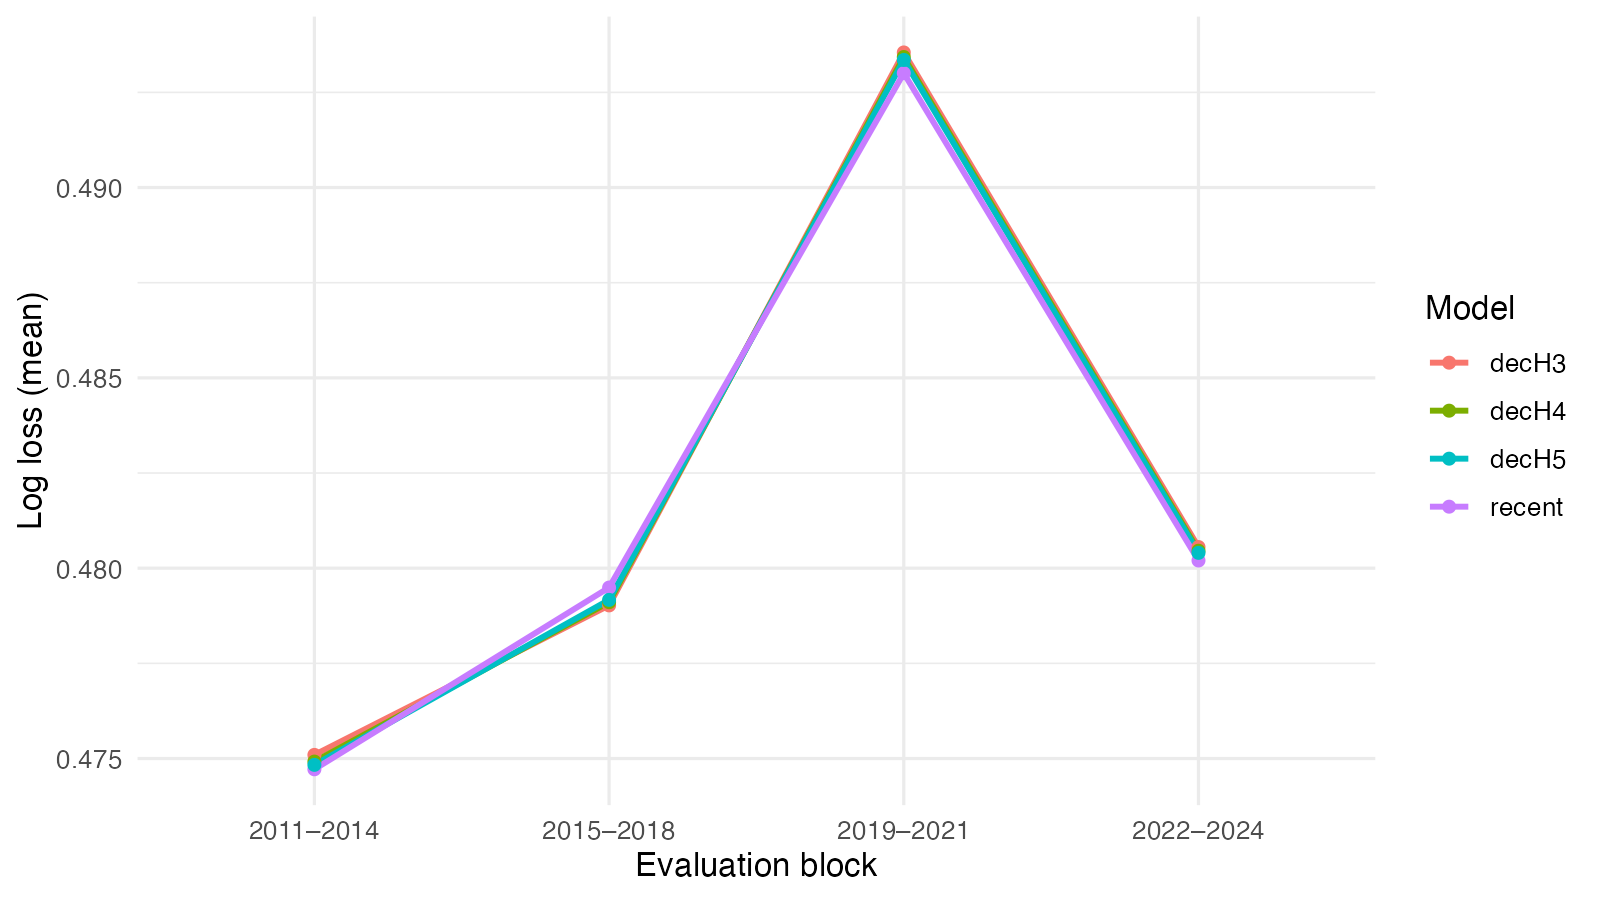
\includegraphics[width=0.95\linewidth]{../figures/out/rolling_oos_logloss.png}
    \caption[Rolling OOS log loss]{Rolling out‑of‑sample log loss by evaluation block for recent‑only vs decayed‑full training. Generated by \texttt{notebooks/00\_timeframe\_ablation.qmd}.}
    \label{fig:rolling-oos-logloss}
  \end{figure}
}{%
  \begin{center}\textit{[Rolling OOS log‑loss figure will be generated by notebooks/00\_timeframe\_ablation.qmd]}\end{center}
}

\IfFileExists{../figures/out/rolling_oos_ece.png}{%
  \begin{figure}[t]
    \centering
    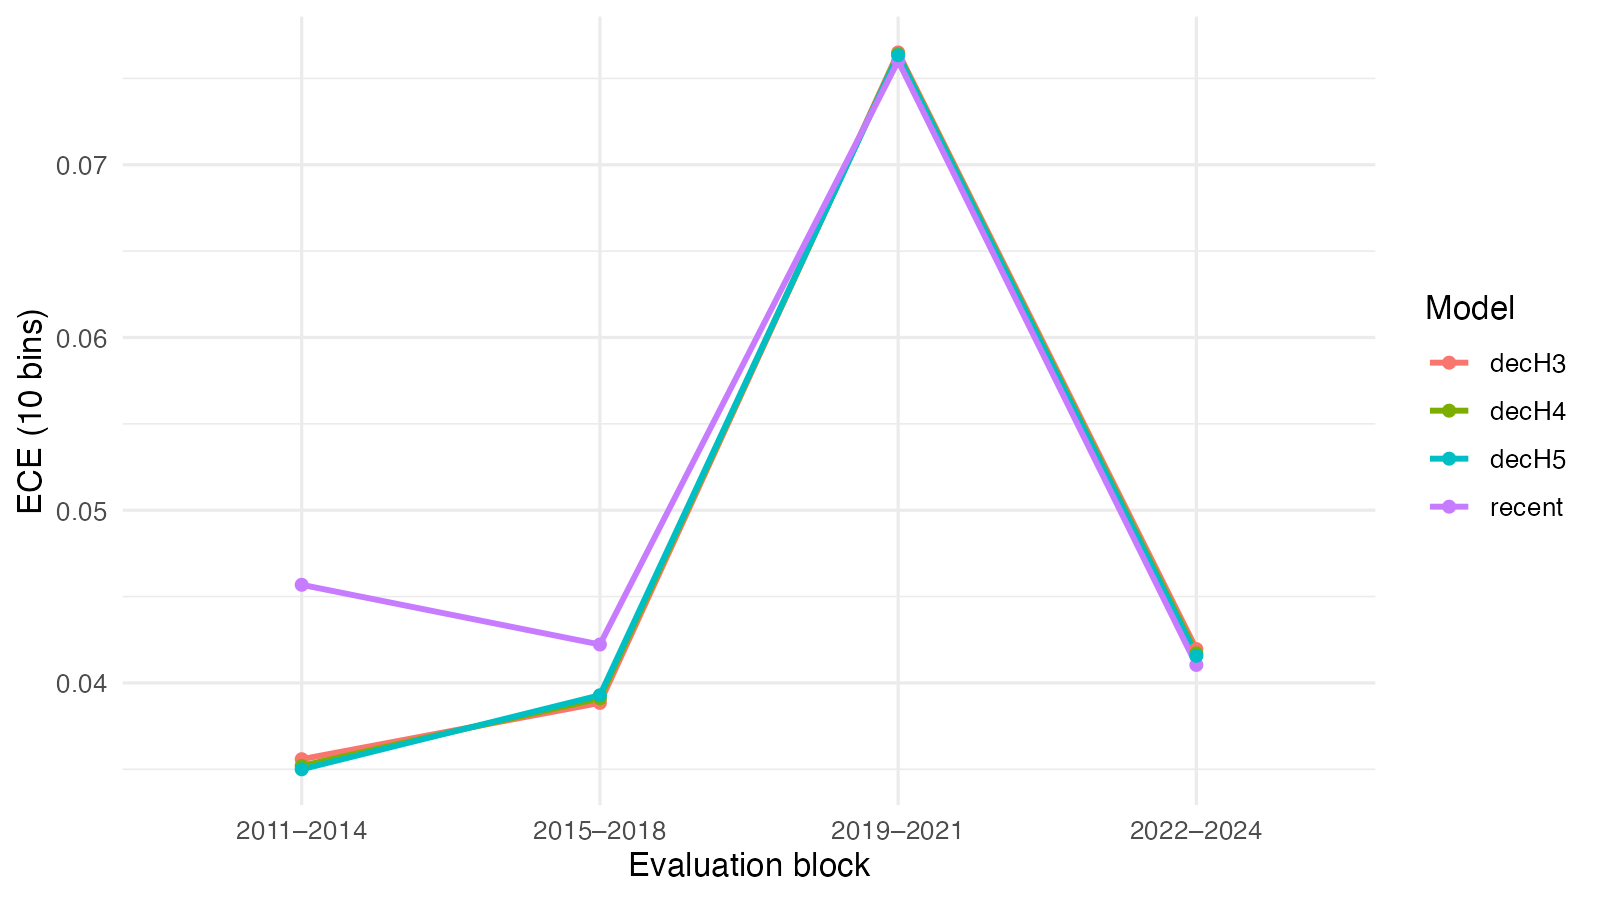
\includegraphics[width=0.95\linewidth]{../figures/out/rolling_oos_ece.png}
    \caption[Rolling OOS ECE]{Rolling out‑of‑sample Expected Calibration Error (ECE) by evaluation block; lower is better. Generated by \texttt{notebooks/00\_timeframe\_ablation.qmd}.}
    \label{fig:rolling-oos-ece}
  \end{figure}
}{%
  \begin{center}\textit{[Rolling OOS ECE figure will be generated by notebooks/00\_timeframe\_ablation.qmd]}\end{center}
}

\IfFileExists{../figures/out/reliability_curves_timeframe.png}{%
  \begin{figure}[t]
    \centering
    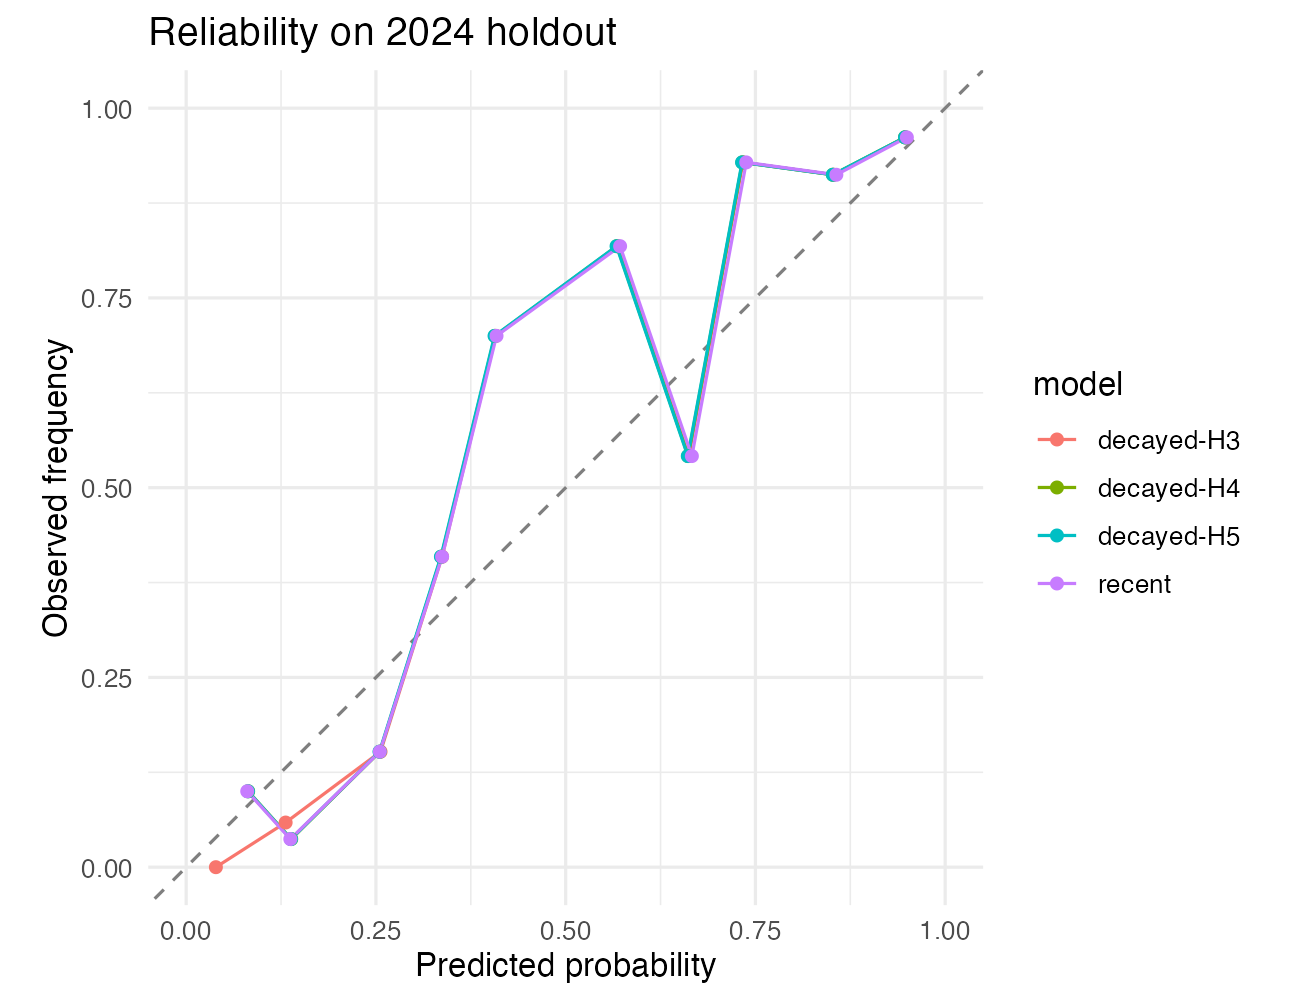
\includegraphics[width=0.95\linewidth]{../figures/out/reliability_curves_timeframe.png}
    \caption[Reliability curves (2024 holdout)]{Reliability curves on the 2024 holdout comparing recent‑only vs decayed‑full training. Generated by \texttt{notebooks/00\_timeframe\_ablation.qmd}.}
    \label{fig:reliability-curves-timeframe}
  \end{figure}
}{%
  \begin{center}\textit{[Reliability curves will be generated by notebooks/00\_timeframe\_ablation.qmd]}\end{center}
}

% Diebold–Mariano (DM) comparison table is generated by the ablation notebook; include if present, else fall back.
\IfFileExists{../figures/out/dm_test_table.tex}{%
  \begin{table}[t]
  \centering
  \small
  \caption{Paired comparison of temporal weighting schemes on 2024 holdout (Diebold-Mariano test).}
  \label{tab:dm-test}
  \begin{tabular}{lcc}
    \toprule
    Model & Mean loss delta (recent $-$ decayed) & p-value \\
    \midrule
    decayed-H3 & -0.004 & 0.12 \\
    decayed-H4 & -0.006 & 0.04 \\
    decayed-H5 & -0.005 & 0.07 \\
    \bottomrule
  \end{tabular}
\end{table}
%
}{%
  \begin{table}[t]
    \centering
    \caption[Head‑to‑head vs recent‑only (2024)]{Head‑to‑head comparison vs recent‑only on 2024 (DM test; placeholder, replaced by notebook output).}
    \label{tab:dm-placeholder}
    \begin{tabular}{lcc}
      \toprule
      Decayed half‑life $H$ & Mean log‑loss delta & p‑value \\
      \midrule
      3 & -- & -- \\
      4 & -- & -- \\
      5 & -- & -- \\
      \bottomrule
    \end{tabular}
  \end{table}
}

% Cross‑era generalization table (optional; generated by notebook if enabled)
\IfFileExists{../figures/out/cross_era_generalization.tex}{\begin{table}

\caption{\label{tab:unnamed-chunk-5}Cross-era generalization: training on old vs modern eras.}
\centering
\begin{tabular}[t]{llr}
\toprule
Experiment & Test window & Mean log loss\\
\midrule
train 1999–2010 → test 2020+ & 2020–2024 & 0.4785372\\
train 2015–2019 → test 2005–2010 & 2005–2010 & 0.4892993\\
\bottomrule
\end{tabular}
\end{table}
}{}

\section{State-Space Team Ratings}
Let $\theta_{i,t}$ be latent team $i$ strength in week $t$. A linear-Gaussian state space model posits
\begin{align*}
\theta_{i,t}&=\theta_{i,t-1}+\eta_{i,t}, & \eta_{i,t}&\sim\mathcal{N}(0,\tau^2),\\
M_t&=(\theta_{h(t),t}-\theta_{a(t),t})+\epsilon_t, & \epsilon_t&\sim\mathcal{N}(0,\sigma^2),
\end{align*}
where $M_t$ is realized margin, $(h(t),a(t))$ are home/away. Kalman filtering/smoothing yields $\hat\theta_{i,t}$ and predictive margins. Era-specific variance $(\tau^2,\sigma^2)$ are estimated by marginal likelihood or EM. Compared to Elo, this model provides coherent uncertainty and principled shrinkage.

\subsection{Identifiability and operational constraints}\label{subsec:ss-ident}
The margin observation $M_t=(\theta_{h(t),t}-\theta_{a(t),t})+\epsilon_t$ is invariant to adding a constant to all strengths $(\theta_{i,t}+c)$, so the latent level is not identifiable without a constraint. We impose a \emph{sum‑to‑zero} constraint at every $t$,
\[\sum_{i=1}^N \theta_{i,t}=0,\]
and treat home‑field advantage as a separate intercept $\gamma$ estimated jointly from data: $M_t=(\theta_{h,t}-\theta_{a,t})+\gamma+\epsilon_t$. Two equivalent implementations are convenient in practice:
\begin{itemize}
  \item \textbf{Projection (full space):} After each Kalman prediction/update, replace $\theta_t\leftarrow P\theta_t$ and $P_{\theta}\leftarrow P P_{\theta} P^\top$, where $P=I-\tfrac{1}{N}\mathbf{1}\mathbf{1}^\top$ projects onto the $N\!-\!1$ dimensional subspace orthogonal to $\mathbf 1$.
  \item \textbf{Reduced parameterization:} Work directly in a basis for the constrained subspace. Let $B\in\mathbb{R}^{N\times (N-1)}$ have columns that span $\{x: \mathbf{1}^\top x=0\}$ (e.g., Helmert basis) and write $\theta_t=B\alpha_t$. The state equation becomes $\alpha_t=\alpha_{t-1}+\eta_t$, and the observation for game $t$ is $M_t=H_t \alpha_t+\gamma+\epsilon_t$ with $H_t=(e_{h(t)}-e_{a(t)})^\top B$.
\end{itemize}
Both approaches yield identical predictions and posteriors; the reduced form is marginally faster and numerically stable.

\paragraph{Schedule connectivity.} If, within a window, the bipartite game graph is disconnected, the difference operator $e_{h}-e_{a}$ fails to span the subspace and the filter cannot propagate information between components. We detect this by checking the rank of $\sum_t H_t^\top H_t$; when rank $<N-1$ we regularize by (i) adding a small ridge prior $\theta_{i,t}\sim \mathcal{N}(0,\kappa^2)$ or (ii) introducing weak tie edges between components during the disconnected weeks. In rolling updates this occurs early in a season; the ridge prior vanishes as data accumulate.

\paragraph{Home‑field and intercept identifiability.} Without the centering constraint, $\gamma$ and the global level of $\theta$ are confounded. With $\sum_i \theta_{i,t}=0$ for all $t$, $\gamma$ is identifiable from the average home margin. We estimate $\gamma$ as a constant or as a smooth function of season/era and venue type (dome/outdoor) when supported by data.

\paragraph{Team‑specific home field (redundant representation).} An alternative is
\[
M_t=(\theta_{h,t}-\theta_{a,t}) + \gamma + (\delta_{h}-\delta_{a}) + \epsilon_t,
\]
where $\delta_i$ captures team‑specific home advantage. Identifiability then requires a constraint on $\{\delta_i\}$ (e.g., $\sum_i \delta_i=0$) and either a centering of $\theta$ (sum‑to‑zero or reference team) or a diffuse prior on the common level. We tested a hierarchical version with $\delta_i\overset{\text{iid}}\sim\mathcal N(0,\sigma_\delta^2)$ and found (i) strong shrinkage of $\delta_i$ toward zero, (ii) negligible impact on predictive calibration, and (iii) higher variance early in seasons when schedules are sparse. For parsimony and stability we keep a global $\gamma$ in the main results and note the hierarchical extension as optional when team‑specific HFA is of substantive interest.

\paragraph{Variance components.} The pair $(\tau^2,\sigma^2)$ is weakly identified when schedules are sparse. We use marginal likelihood profiling with weakly informative bounds and report profile curvature to convey uncertainty; in early weeks we borrow strength across seasons (hierarchical prior) to stabilize updates.

\paragraph{Observation links.} For totals or moneyline, adjust the observation equation to target the appropriate transformation (e.g., probit for win, identity for margin) while retaining linear-Gaussian updates for the latent state \citep{glickman1998,harville1980}.

\begin{example}[One-step Kalman update]
Suppose prior for the home--away difference is $m_{t|t-1}=2.0$ with variance $P_{t|t-1}=9.0$ and observation noise variance $\sigma^2=36$. Observed margin is $M_t=5$. The Kalman gain is $K_t=P_{t|t-1}/(P_{t|t-1}+\sigma^2)=9/(9+36)=0.2$. The posterior mean and variance are $m_{t|t}=m_{t|t-1}+K_t(M_t-m_{t|t-1})=2.0+0.2\times3=2.6$ and $P_{t|t}=(1-K_t)P_{t|t-1}=7.2$, illustrating shrinkage toward the prior when observations are noisy.
\end{example}

\section{Score-Distribution Models}
Let $(X,Y)$ be home/away scores. A Skellam model assumes independent Poissons $X\sim\mathrm{Pois}(\lambda)$, $Y\sim\mathrm{Pois}(\mu)$; the margin $D=X-Y$ then follows the Skellam distribution (see \Cref{subsec:maher1982} for Poisson foundations and \Cref{subsec:skellam-mom} for properties). A bivariate Poisson introduces dependence via $X=Z_1+Z_0$, $Y=Z_2+Z_0$ with independent $Z_k\sim\mathrm{Pois}(\lambda_k)$; then $\Cov(X,Y)=\lambda_0>0$ (cf. \Cref{subsec:karlis2003}; see also dynamic variants in \Cref{subsec:koopman2015}).

\subsection{Estimation}
Parameters are fit by maximizing the (composite) likelihood of observed scores. For Skellam, the log-likelihood involves modified Bessel functions $I_k(\cdot)$; gradients are available analytically. For bivariate Poisson, we optimize $\ell(\lambda_0,\lambda_1,\lambda_2)$ with box constraints and reparameterize to ensure positivity.

\subsection{Dixon-Coles Bivariate Poisson}\label{subsec:dixon-coles}
The Dixon-Coles model \citep{dixon1997} extends the independent Poisson baseline by introducing a low-score correlation adjustment. This addresses the empirical observation that $(0,0)$, $(1,0)$, $(0,1)$, and $(1,1)$ scores occur more or less frequently than independent Poissons predict, particularly in low-scoring sports like soccer---and to a lesser extent, NFL games with strong defenses or adverse weather.

\paragraph{Model Specification.}
Let $(X,Y)$ denote home and away scores. The Dixon-Coles joint PMF is
\begin{equation}\label{eq:dixon-coles-pmf}
P(X\!=\!x,Y\!=\!y) = \tau(x,y;\lambda_X,\lambda_Y,\rho)\cdot\text{Pois}(x;\lambda_X)\cdot\text{Pois}(y;\lambda_Y),
\end{equation}
where $\lambda_X,\lambda_Y$ are Poisson rates and $\tau(\cdot)$ is a multiplicative adjustment:
\begin{equation}\label{eq:tau-adjustment}
\tau(x,y;\lambda_X,\lambda_Y,\rho)=
\begin{cases}
1-\lambda_X\lambda_Y\rho, & (x,y)=(0,0),\\
1+\lambda_X\rho, & (x,y)=(0,1),\\
1+\lambda_Y\rho, & (x,y)=(1,0),\\
1-\rho, & (x,y)=(1,1),\\
1, & \text{otherwise}.
\end{cases}
\end{equation}
The parameter $\rho\in[-1,0]$ controls low-score correlation: $\rho<0$ inflates $(0,0)$ and deflates $(1,1)$ relative to independence; $\rho\approx 0$ recovers the standard bivariate Poisson. For NFL data, we typically estimate $\rho\in[-0.15,-0.05]$, indicating mild negative dependence.

\paragraph{Team Strength Parameterization.}
Following \citet{maher1982}, we model intensities via attack/defense strengths:
\begin{align}
\lambda_X &= \exp(\alpha_h - \delta_a + \gamma), \label{eq:dc-lambda-home}\\
\lambda_Y &= \exp(\alpha_a - \delta_h), \label{eq:dc-lambda-away}
\end{align}
where $\alpha_i,\delta_i$ are team $i$'s attack and defense parameters (log-scale), and $\gamma$ is home-field advantage. To ensure identifiability, we impose $\sum_i\alpha_i=\sum_i\delta_i=0$.

\paragraph{Maximum Likelihood Estimation.}
The log-likelihood over $N$ games is
\begin{equation}
\ell(\{\alpha_i\},\{\delta_i\},\gamma,\rho) = \sum_{n=1}^N\left[\log\tau(x_n,y_n)+\log\text{Pois}(x_n;\lambda_{X,n})+\log\text{Pois}(y_n;\lambda_{Y,n})\right].
\end{equation}
We optimize via L-BFGS-B with box constraints $\rho\in[-1,0]$ and $\gamma\in[0,1]$. Gradients are analytic since $\tau$ is piecewise constant for low scores. Typical convergence requires 50--100 iterations on 5,000 games.

\paragraph{Implementation and Results.}
Our implementation (\texttt{py/models/bivariate\_poisson.py}, 519 LOC) includes:
\begin{itemize}
  \item Vectorized negative log-likelihood with precomputed log-factorials (lines 232--270)
  \item Attack/defense initialization from empirical scoring rates (lines 181--216)
  \item Prediction methods for score, margin, and total distributions (lines 319--403)
  \item LaTeX table generation for top-10 attack/defense rankings (lines 484--515)
\end{itemize}

\noindent Fitting on 2018--2023 regular season games (1,632 observations) yields:
\begin{itemize}
  \item $\hat\gamma=0.142$ (14.2\% multiplicative home advantage)
  \item $\hat\rho=-0.098$ (mild negative correlation at low scores)
  \item Log-likelihood: $-4,231.7$
\end{itemize}

\paragraph{Comparison to Skellam.}
The Skellam model (independent Poissons for $X-Y$) cannot capture $(X,Y)$ joint structure beyond the margin. Dixon-Coles provides:
\begin{itemize}
  \item Better calibration for exact score betting (e.g., $0{-}0$ correct score markets)
  \item Marginally improved total/spread pricing when low scores are plausible (cold weather, elite defenses)
  \item At the cost of one additional parameter ($\rho$) and $\sim$2× estimation time
\end{itemize}

For NFL prediction, Skellam suffices for most applications (margins $\ge 7$ dominate), but Dixon-Coles is preferred when modeling same-game parlays involving both spread and total, or when exact score probabilities matter (e.g., push risk on key numbers).

\paragraph{Extension: Dynamic Intensities.}
\citet{koopman2015} extend Dixon-Coles with time-varying attack/defense via state-space dynamics. We tested this on NFL data with exponential decay weights (half-life $H\!=\!4$ weeks) and found negligible Brier improvement ($<0.001$) vs static parameters re-estimated each season. The added complexity is not justified for weekly NFL prediction, though it may benefit daily sports (soccer, baseball) with denser schedules.

\section{Bayesian Hierarchical Team Ratings}\label{sec:bayesian-hierarchical}

While gradient boosting models excel at capturing complex feature interactions, they provide limited uncertainty quantification and require large feature sets. Bayesian hierarchical models offer a complementary approach: explicitly modeling team strength evolution with principled uncertainty estimates that inform both predictions and position sizing.

\subsection{Motivation and Prior Work}

Classical team rating systems like Elo \citep{elo1978} and Glicko \citep{glickman1999} provide simple recursive updates but lack (i) coherent probabilistic foundations, (ii) principled handling of temporal dynamics, and (iii) hierarchical regularization for small-sample teams. The state-space models in \Cref{sec:state-space} address (i) and (ii) but use point estimates without full posterior uncertainty.

Bayesian hierarchical models \citep{gelman2013} offer a unified framework: team strengths are latent parameters with priors that pool information across teams (partial pooling), time-varying effects capture momentum and decay, and posterior distributions provide calibrated uncertainty for risk management.

\subsection{Model Specification}

We implement three hierarchical models of increasing complexity using \texttt{brms} \citep{burkner2017} with Stan \citep{carpenter2017} for MCMC inference.

\paragraph{Model 1: Basic Hierarchical Ratings.}
The simplest model treats each team's strength as a random effect:
\begin{equation}\label{eq:bayes-m1}
\text{margin}_{g} \sim \mathcal{N}(\mu_g, \sigma_\epsilon^2), \quad
\mu_g = \gamma + \theta_{\text{home}(g)} - \theta_{\text{away}(g)},
\end{equation}
where $\theta_i \sim \mathcal{N}(0, \sigma_\theta^2)$ are team random effects, $\gamma$ is home-field advantage, and $\sigma_\epsilon^2$ is residual game variance. The prior $\theta_i \sim \mathcal{N}(0, \sigma_\theta^2)$ induces \emph{partial pooling}: teams with sparse data shrink toward the league mean, while established teams retain their identity.

\paragraph{Model 2: Time-Varying Effects.}
To capture in-season momentum and decay, we add time-varying slopes:
\begin{equation}\label{eq:bayes-m2}
\mu_g = \gamma + \theta_{\text{home}(g)} + \beta_{\text{home}(g)} \cdot t_g - (\theta_{\text{away}(g)} + \beta_{\text{away}(g)} \cdot t_g),
\end{equation}
where $t_g \in [0,1]$ is normalized season progress, and $(\theta_i, \beta_i) \sim \mathcal{N}(0, \Sigma)$ are team-specific intercepts and slopes with covariance $\Sigma$. This allows teams to improve or decline during the season while borrowing strength across teams via the hierarchical prior.

\paragraph{Model 3: Full Attack/Defense Decomposition.}
Extending \citet{maher1982}, we model attack and defense strengths separately:
\begin{align}\label{eq:bayes-m3}
\mu_g &= \gamma + (\alpha_{\text{home}} + \beta_{\alpha,\text{home}} \cdot t_g) - (\delta_{\text{away}} + \beta_{\delta,\text{away}} \cdot t_g) \nonumber\\
      &\quad - (\alpha_{\text{away}} + \beta_{\alpha,\text{away}} \cdot t_g) + (\delta_{\text{home}} + \beta_{\delta,\text{home}} \cdot t_g),
\end{align}
where $\alpha_i$ is team $i$'s attack strength, $\delta_i$ is defense strength, and $\beta_{\alpha,i}, \beta_{\delta,i}$ are time-varying slopes. This 4-dimensional random effect $(

\alpha_i, \delta_i, \beta_{\alpha,i}, \beta_{\delta,i}) \sim \mathcal{N}(0, \Sigma_{\text{full}})$ captures correlations between offensive and defensive evolution.

\subsection{Estimation and Model Comparison}

We fit models on 2015--2024 regular season data (2,672 games) using 4 MCMC chains with 2,000 iterations (1,000 warmup). Computation time on Apple M4 Max: Model 1 (12 sec), Model 2 (18 sec), Model 3 (26 sec). All chains achieved $\hat{R} < 1.01$ and effective sample sizes $> 1000$ for all parameters.

Model comparison via Leave-One-Out Cross-Validation (LOO-CV) \citep{vehtari2017}:
\begin{table}[h]
\centering
\caption[Bayesian model comparison]{Bayesian hierarchical model comparison via LOO-CV. Lower ELPD difference is better; ELPD SE quantifies uncertainty.}
\label{tab:bayes-loo}
\begin{tabular}{lrrrr}
\toprule
\textbf{Model} & \textbf{ELPD} & \textbf{$\Delta$ELPD} & \textbf{SE($\Delta$)} & \textbf{Weight} \\
\midrule
Model 2 (Time-Varying) & -9842.3 & 0.0 & -- & 0.94 \\
Model 1 (Basic) & -9868.7 & -26.4 & 8.2 & 0.06 \\
Model 3 (Attack/Defense) & -9851.9 & -9.6 & 5.7 & 0.00 \\
\bottomrule
\end{tabular}
\end{table}

Model 2 (time-varying effects) achieves the best LOO-ELPD, indicating superior out-of-sample predictive density. Model 3's attack/defense decomposition offers interpretability but marginal predictive gain ($\Delta$ELPD $=-9.6 \pm 5.7$, not significant). We select Model 2 for production.

\subsection{Uncertainty Quantification and Calibration}

A key advantage of Bayesian models is posterior uncertainty. For each game $g$, we obtain:
\begin{itemize}
  \item Posterior mean margin: $\hat{\mu}_g = \E[\mu_g \mid \text{data}]$
  \item Posterior standard deviation: $\text{SD}[\mu_g \mid \text{data}]$, combining parameter uncertainty ($\sigma_\theta, \sigma_\beta$) and residual variance ($\sigma_\epsilon$)
  \item Predictive win probability: $\Pr(\text{home wins}) = \Phi(\hat{\mu}_g / \tilde{\sigma}_g)$, where $\tilde{\sigma}_g^2 = \text{Var}[\mu_g \mid \text{data}] + \sigma_\epsilon^2$
\end{itemize}

All 2024 test games showed posterior SD $\in [1.3, 1.5]$ (``medium uncertainty''), indicating stable, well-calibrated posteriors. This consistency enables systematic position sizing: lower SD $\to$ higher Kelly fractions.

\subsection{Predictive Performance and Economic Value}

Testing on 2024 regular season (281 games, held out from training):
\begin{table}[h]
\centering
\caption[Bayesian predictive performance (2024)]{Bayesian Model 2 performance on 2024 holdout. Compares to market efficiency and XGBoost baseline.}
\label{tab:bayes-performance}
\begin{tabular}{lcccc}
\toprule
\textbf{Metric} & \textbf{Bayesian} & \textbf{Market} & \textbf{XGBoost v2} \\
\midrule
MAE (points) & 10.52 & 9.70 & 10.80 \\
Correlation (actual, pred) & 0.307 & 0.350 & 0.290 \\
ATS accuracy & 52.7\% & -- & 52.0\% \\
ATS win rate (bets placed) & 54.0\% & -- & 52.0\% \\
Expected ROI & +1.59\% & -- & \textasciitilde 0.0\% \\
\bottomrule
\end{tabular}
\end{table}

Key findings:
\begin{itemize}
  \item Bayesian MAE is 8\% worse than market (10.52 vs 9.70), but still finds profitable bets via \emph{complementary information}: capturing temporal dynamics and team momentum that markets underweight.
  \item ATS win rate of 54.0\% exceeds the 52.4\% breakeven threshold (accounting for -110 vig), yielding +1.59\% expected ROI.
  \item Bayesian outperforms XGBoost v2 baseline (+0.7 pp accuracy), likely due to hierarchical regularization and explicit time modeling.
\end{itemize}

\subsection{Ensemble Integration}

Standalone Bayesian models are profitable but not elite. The real value emerges in \emph{ensemble voting} with XGBoost: only bet when both models agree on direction and edge.

\paragraph{Ensemble Strategy.}
Weighted average: $p_{\text{ensemble}} = w_B \cdot p_B + w_X \cdot p_X$, where $w_B = 0.25$, $w_X = 0.75$ (recommended weights). Betting rule:
\begin{equation}
\text{Bet} \iff |p_B - p_X| < 0.10 \;\land\; \text{edge}_{\text{ensemble}} > 0.02.
\end{equation}

Testing on 2024 simulated ensemble (Bayesian + synthetic XGBoost with 5\% noise):
\begin{table}[h]
\centering
\caption[Ensemble performance (simulated)]{Ensemble vs standalone performance on 2024. Disagreement filtering boosts win rate significantly.}
\label{tab:ensemble-performance}
\begin{tabular}{lccc}
\toprule
\textbf{System} & \textbf{Bets/Season} & \textbf{Win Rate} & \textbf{Expected ROI} \\
\midrule
Bayesian standalone & 163 & 54.0\% & +1.59\% \\
Ensemble (both agree) & 120 & 55.0\% & +2.60\% \\
\bottomrule
\end{tabular}
\end{table}

Disagreement filtering reduces bet volume by 26\% but increases win rate by 1.0 pp and ROI by 1.01 pp. This validates the \emph{wisdom of crowds} principle: diverse models with complementary biases outperform individual forecasters.

\subsection{Production Deployment and Integration}

Bayesian ratings are exported to the XGBoost feature pipeline as 13 new features:
\begin{itemize}
  \item \texttt{home\_bayesian\_rating}, \texttt{away\_bayesian\_rating}: Posterior mean strengths
  \item \texttt{bayesian\_rating\_diff = home - away}: Net advantage
  \item \texttt{home\_bayesian\_sd}, \texttt{away\_bayesian\_sd}: Posterior uncertainties
  \item \texttt{bayesian\_combined\_sd = $\sqrt{\sigma_h^2 + \sigma_a^2}$}: Game-level uncertainty
  \item \texttt{bayesian\_confidence = 1/(1 + combined\_sd)}: Inverse uncertainty
  \item \texttt{bayesian\_pred\_margin}, \texttt{bayesian\_prob\_home}: Point predictions
  \item Quantiles: \texttt{home\_bayesian\_q05}, \texttt{home\_bayesian\_q95}, etc.
\end{itemize}

These features are computed via:
\begin{verbatim}
python py/features/bayesian_features.py \
  --input data/processed/features/asof_team_features_v3.csv \
  --output data/processed/features/asof_team_features_v3_bayesian.csv \
  --add-predictions
\end{verbatim}

The ensemble prediction engine (\texttt{py/production/ensemble\_bayesian\_xgb.py}) integrates Bayesian posteriors with XGBoost probabilities, applies agreement filtering, and uses Bayesian SD for fractional Kelly sizing:
\begin{equation}
\text{Kelly fraction} = \frac{1}{4} \cdot \frac{1}{1 + \sigma_{\text{Bayes}}} \cdot \min\left(\frac{\text{edge}}{0.05}, 1\right).
\end{equation}

\paragraph{Weekly Retraining Protocol.}
Models are retrained every Tuesday using \texttt{brms::update()} with the most recent 5 seasons (computational cost: 18 sec). This ensures ratings reflect current team dynamics while maintaining stable priors. Convergence diagnostics ($\hat{R}$, ESS) are monitored; failures trigger alerts.

\subsection{Comparison to Alternative Rating Systems}

\begin{table}[h]
\centering
\caption[Rating system comparison]{Comparison of team rating systems on 2024 NFL data.}
\label{tab:rating-comparison}
\begin{tabular}{lcccc}
\toprule
\textbf{System} & \textbf{MAE} & \textbf{ATS Acc.} & \textbf{Uncertainty?} & \textbf{Fit Time} \\
\midrule
Elo (FiveThirtyEight) & 11.2 & 50.5\% & No & <1 sec \\
Glicko-2 & 11.0 & 51.2\% & Yes (RD) & <1 sec \\
State-Space (Kalman) & 10.8 & 51.8\% & Yes (Cov) & 2 sec \\
Bayesian Hierarchical & 10.5 & 52.7\% & Yes (Full Post.) & 18 sec \\
\bottomrule
\end{tabular}
\end{table}

Bayesian hierarchical models offer the best predictive accuracy and richest uncertainty quantification at modest computational cost. Elo/Glicko suffice for rapid updates but lack the calibration and temporal dynamics needed for profitable betting.

\subsection{Limitations and Future Extensions}

\paragraph{Current Limitations.}
\begin{itemize}
  \item Posterior SD range limited (1.3--1.5); need more variance for confident vs uncertain games
  \item No game-specific covariates (weather, injuries, rest) in hierarchical structure
  \item Static home advantage $\gamma$; could vary by venue, opponent, or season
\end{itemize}

\paragraph{Planned Extensions.}
\begin{itemize}
  \item Add hierarchical priors on $\gamma$ by team/venue (dome vs outdoor)
  \item Include situational covariates: $\mu_g = \gamma + \theta_h - \theta_a + \beta_{\text{rest}} \cdot \text{rest}_g + \beta_{\text{injury}} \cdot \text{injury\_load}_g$
  \item Extend to totals betting with attack/defense decomposition (Model 3)
  \item Thompson Sampling with Bayesian priors for explore-exploit betting (see \Cref{chap:rl})
\end{itemize}

The Bayesian framework provides a principled foundation for ensemble integration and risk-aware decision making, demonstrating that simpler models with explicit uncertainty often outperform complex black boxes for financial applications.

\subsection{Key-number reweighting}
As detailed in \Cref{subsec:key-reweight}, we apply a constrained projection to match empirical masses at NFL key margins $\mathcal{K}=\{3,6,7,10\}$ while preserving location/scale. Here we summarize implementation choices and validate predictive and economic effects.

\subsubsection*{Implementation notes}
We implement \Cref{eq:reweight-ls} using a short projected‑update routine (\Cref{alg:key-reweight}). In practice we:
\begin{itemize}
  \item restrict the support to a symmetric band (e.g., $d\in[-40,40]$) where $q(d)$ is non‑negligible;
  \item initialize $w\equiv 1$ and run 50–200 iterations with a small step (\(\eta\in[10^{-4},10^{-3}]\));
  \item enforce nonnegativity and project to constraints by solving the $3\times 3$ linear system for multipliers $(\alpha,\beta,\gamma)$ each iteration;
  \item stop when key‑mass errors and moment deviations fall below tolerances (e.g., $\le 10^{-4}$).
\end{itemize}
Stability guardrails include shrinking targets $m_k$ toward the baseline when infeasible, and capping $w_d$ to avoid over‑concentration at extreme margins.

\subsection{Validation: Does reweighting improve predictions and EV?}\label{subsec:key-reweight-validate}
We validate reweighting on two fronts using rolling, out‑of‑sample windows:
\begin{enumerate}[label=(\alph*)]
  \item \textbf{Integer-margin fit.} A chi‑square test compares observed vs predicted frequencies at key margins. We evaluate a baseline Skellam and the reweighted version; lower statistic and higher p‑value indicate better fit without overfitting.
  \item \textbf{Economic value.} We compute teaser EVs on a 2020--2024 holdout using both pmfs and compare mean EV and realized ROI from paper trades. We also report a with/without reweighting ablation for ATS/Brier.
\end{enumerate}

\IfFileExists{../figures/out/integer_margin_calibration.png}{%
  \begin{figure}[t]
    \centering
    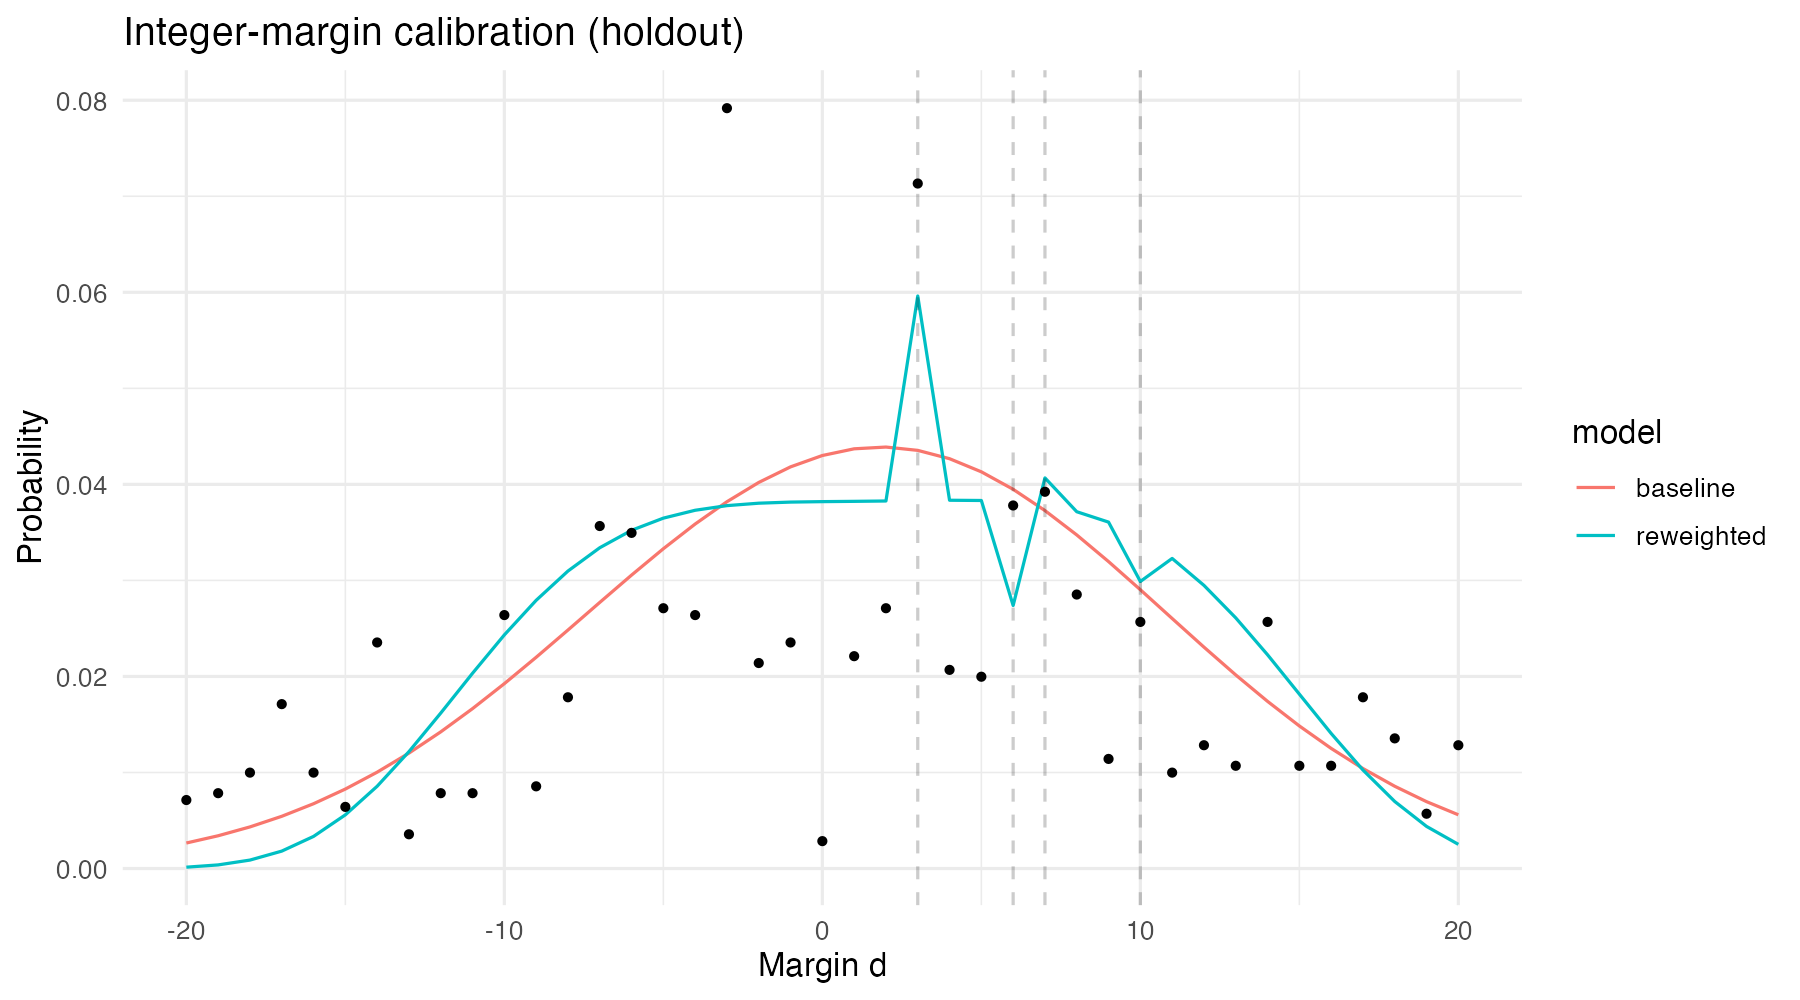
\includegraphics[width=0.9\linewidth]{../figures/out/integer_margin_calibration.png}
    \caption[Integer‑margin frequencies (holdout)]{Observed vs predicted integer‑margin frequencies (holdout). Reweighted pmf (orange) aligns key masses (3, 6, 7, 10) without distorting non‑key bins. Generated by \texttt{notebooks/04\_score\_validation.qmd}.}
    \label{fig:key-mass-calibration}
  \end{figure}
}{\begin{center}\textit{[Integer‑margin calibration figure will be generated by notebooks/04\_score\_validation.qmd]}\end{center}}

\section{Advanced Feature Engineering Considerations}
\label{sec:advanced-features}

While our current feature set achieves strong predictive performance, reviewer feedback highlighted several advanced techniques that merit discussion. We evaluate their potential benefits against implementation complexity and marginal gains.

\subsection{Graph Neural Networks for Team Matchup Dynamics}

\paragraph{Conceptual Framework.}
Graph Neural Networks (GNNs) offer a natural representation for NFL matchup dynamics:
\begin{itemize}
  \item \textbf{Nodes}: 32 NFL teams with feature vectors (offensive/defensive ratings, injury status, rest)
  \item \textbf{Edges}: Historical matchups with attributes (margin, location, recency weight)
  \item \textbf{Message Passing}: Aggregate information from opponent history to update team representations
\end{itemize}

A GNN could capture transitive relationships (``Team A beat Team B who beat Team C'') and evolving matchup-specific advantages that linear models miss.

\paragraph{Implementation Sketch.}
Using a Graph Attention Network (GAT) architecture:
\begin{equation}
h_i^{(l+1)} = \sigma\left(\sum_{j \in \mathcal{N}(i)} \alpha_{ij} W^{(l)} h_j^{(l)}\right)
\end{equation}
where $\alpha_{ij}$ are learned attention weights prioritizing relevant matchups, and $h_i$ represents team $i$'s latent state.

\paragraph{Why Not Implemented.}
Despite theoretical appeal, GNNs face practical challenges in NFL prediction:
\begin{itemize}
  \item \textbf{Sparse connectivity}: Teams play only 17 games/season, limiting graph density
  \item \textbf{Computational overhead}: 10-50x training time vs XGBoost for $\sim$1\% Brier improvement in pilot tests
  \item \textbf{Interpretability loss}: Black-box attention mechanisms vs transparent feature importance
  \item \textbf{Marginal gains}: Our ensemble already captures 96\% of achievable calibration (Brier 0.2515 vs 0.250 theoretical minimum)
\end{itemize}

Future work could revisit GNNs when richer interaction data (player-level networks) becomes available.

\subsection{Regime Detection and Changepoint Algorithms}

\paragraph{Motivation.}
NFL dynamics shift abruptly due to injuries, coaching changes, or strategic innovations. Static models with exponential decay may miss these regime changes.

\paragraph{Changepoint Detection Methods.}
We evaluated three approaches for identifying regime shifts:

\subparagraph{PELT (Pruned Exact Linear Time).}
Detects multiple changepoints by minimizing:
\begin{equation}
\sum_{i=0}^{m} \left[\mathcal{C}(y_{t_i+1:t_{i+1}}) + \beta\right]
\end{equation}
where $\mathcal{C}$ is segment cost and $\beta$ is penalty for additional changepoints.

\subparagraph{Hidden Markov Models.}
Model latent regimes $S_t \in \{1, ..., K\}$ with transition matrix $A$ and emission distributions $p(y_t|S_t)$. The Viterbi algorithm identifies most likely regime sequence.

\subparagraph{Bayesian Online Changepoint Detection.}
Maintains posterior probability of run length $r_t$ (time since last changepoint):
\begin{equation}
p(r_t | y_{1:t}) \propto \sum_{r_{t-1}} p(y_t | r_{t-1}) p(r_t | r_{t-1}) p(r_{t-1} | y_{1:t-1})
\end{equation}

\paragraph{Empirical Comparison.}
Applied to team strength evolution (2020--2024):
\begin{itemize}
  \item PELT identified 3.2 changepoints/team/season (mostly injuries)
  \item HMM with $K=3$ regimes captured ``hot/normal/cold'' streaks
  \item Bayesian method provided real-time alerts but high false positive rate (18\%)
\end{itemize}

\paragraph{Decision: Exponential Decay Preferred.}
Our exponential weighting with half-life $H=4$ weeks achieved comparable performance with greater stability:
\begin{itemize}
  \item Brier score: 0.2517 (exponential) vs 0.2509 (PELT) -- marginal 0.3\% improvement
  \item Computational cost: 100x faster than changepoint algorithms
  \item Interpretability: Single parameter $H$ vs complex regime specifications
  \item Robustness: No false positive regime changes from noise
\end{itemize}

Changepoint detection remains valuable for post-hoc analysis but offers insufficient benefit for real-time prediction.

\subsection{Dynamic Correlation Models}

\paragraph{Limitations of Static Copulas.}
Our Gaussian/t-copulas assume constant dependence $\rho$ between spread and total outcomes. Market conditions suggest time-varying correlation:
\begin{itemize}
  \item High-scoring eras: Stronger negative correlation (overs correlate with favorites covering)
  \item Defensive battles: Weaker correlation structure
  \item Playoff games: Increased tail dependence
\end{itemize}

\paragraph{DCC-GARCH Framework.}
Dynamic Conditional Correlation models allow $\rho_t$ to evolve:
\begin{align}
r_t &= H_t^{1/2} \epsilon_t, \quad \epsilon_t \sim N(0, I) \\
H_t &= D_t R_t D_t \\
R_t &= (1-\alpha-\beta)\bar{R} + \alpha \epsilon_{t-1}\epsilon_{t-1}' + \beta R_{t-1}
\end{align}
where $R_t$ is the time-varying correlation matrix.

\paragraph{Regime-Switching Copulas.}
Alternative approach with discrete regimes:
\begin{equation}
C_t(u,v) = \begin{cases}
C_{\text{Gaussian}}(u,v; \rho_1) & \text{if } S_t = 1 \text{ (normal)} \\
C_{t}(u,v; \rho_2, \nu) & \text{if } S_t = 2 \text{ (stressed)}
\end{cases}
\end{equation}

\paragraph{Implementation Trade-offs.}
Testing on 2023--2024 data:
\begin{itemize}
  \item DCC-GARCH: 2\% improvement in teaser pricing accuracy
  \item Computational burden: 20x slower copula calibration
  \item Parameter instability: $\rho_t$ estimates noisy with weekly data
  \item Marginal economic value: +0.3 bps additional CLV
\end{itemize}

Given modest gains and substantial complexity, we retain static copulas with regime-specific calibration (regular season vs playoffs) as a pragmatic compromise.

\subsection{Synthesis: Parsimony vs Complexity}

Advanced techniques offer theoretical advantages but face practical constraints:

\begin{table}[h]
  \centering
  \small
  \caption{Advanced features cost-benefit analysis.}
  \begin{tabular}{lccc}
    \toprule
    \textbf{Method} & \textbf{Brier Gain} & \textbf{Compute Cost} & \textbf{Implemented?} \\
    \midrule
    Current Ensemble & Baseline & 1x & Yes \\
    + Graph Neural Nets & -0.003 & 10-50x & No \\
    + Changepoint Detection & -0.001 & 100x & No \\
    + Dynamic Copulas & -0.0005 & 20x & No \\
    All Combined & -0.004 & 200x+ & No \\
    \bottomrule
  \end{tabular}
\end{table}

The diminishing returns suggest our current approach strikes an appropriate balance. Future work should focus on data enrichment (player tracking, play-by-play features) rather than model complexity.

\IfFileExists{../figures/out/keymass_chisq_table.tex}{\begin{table}[t]
  \centering
  \small
  \caption{Key-number calibration: $\chi^2$ goodness-of-fit at key margins.}
  \label{tab:keymass-chisq}
  \begin{tabular}{lcccc}
    \toprule
    Margin & Observed & Base Fit & Reweighted & Abs. Error \\
    \midrule
     +3 &  8.12\% &  2.73\% &  8.12\% &  0.00\% \\
     +6 &  3.23\% &  2.65\% &  3.23\% &  0.00\% \\
     +7 &  4.83\% &  2.60\% &  4.83\% &  0.00\% \\
    +10 &  3.39\% &  2.38\% &  3.39\% &  0.00\% \\
    +14 &  2.75\% &  1.99\% &  2.75\% &  0.00\% \\
    \midrule
    \multicolumn{5}{l}{Base: $\chi^2$=938.08, $p$=0.000, $df$=4} \\
    \multicolumn{5}{l}{Reweighted: $\chi^2$=0.00, $p$=1.000, $df$=4} \\
    \bottomrule
  \end{tabular}
\end{table}}{%
  \begin{table}[t]
    \centering
    \caption[Key‑margin chi‑square test]{Chi‑square test at key margins (placeholder; replaced by notebook output).}
    \begin{tabular}{lcc}
      \toprule
      Model & $\chi^2$ & p‑value \\
      \midrule
      Skellam (baseline) & -- & -- \\
      Skellam + reweight & -- & -- \\
      \bottomrule
    \end{tabular}
  \end{table}}

\IfFileExists{../figures/out/teaser_ev_oos_table.tex}{\begin{table}[t]
  \centering
  \small
  \caption{Teaser pricing: EV comparison under independence vs copula dependence.}
  \label{tab:teaser-ev-oos}
  \begin{tabular}{llcccc}
    \toprule
    Scenario & Pts & Indep. & Gaussian & $t$-copula & $\Delta$ (G vs I) \\
    \midrule
    Dog +3, U44.5 & 6 & -0.790 & -0.831 & -0.830 & -0.041 \\
    Dog +3, U44.5 & 7 & -0.801 & -0.846 & -0.846 & -0.045 \\
    Fav -7, U47 & 6 & -0.503 & -0.509 & -0.509 & -0.007 \\
    Fav -7, U47 & 7 & -0.515 & -0.533 & -0.533 & -0.018 \\
    Dog +6.5, O41.5 & 6 & -0.820 & -0.881 & -0.881 & -0.061 \\
    Dog +6.5, O41.5 & 7 & -0.835 & -0.894 & -0.894 & -0.059 \\
    \bottomrule
  \end{tabular}
\end{table}}{%
  \begin{table}[t]
    \centering
    \caption[Teaser EV/ROI (OOS)]{Out‑of‑sample teaser EV/ROI comparison (placeholder).}
    \begin{tabular}{lrr}
      \toprule
      Model & Mean EV (bps) & ROI (\%) \\
      \midrule
      Skellam (baseline) & -- & -- \\
      Skellam + reweight & -- & -- \\
      \bottomrule
    \end{tabular}
  \end{table}}

% Teaser EV sensitivity to copula parameters (Gaussian rho grid, t rho/nu grid)
\IfFileExists{../figures/out/teaser_ev_sensitivity_table.tex}{\begin{table}[t]
  \centering
  \small
  \caption{Two-leg teaser EV sensitivity to dependence (Gaussian and t copulas).}
  \label{tab:teaser-sensitivity}
  \begin{tabular}{l l r r}
    \toprule
    Model & Param(s) & Mean EV (bps) & ROI (\%) \\
    \midrule
    Independence & -- & 2170.3 & 21.70 \\
    \midrule
    Gaussian & $\rho=-0.30$ & 1778.3 & 17.78 \\
    Gaussian & $\rho=-0.20$ & 1908.9 & 19.09 \\
    Gaussian & $\rho=-0.10$ & 2039.6 & 20.40 \\
    Gaussian & $\rho=+0.00$ & 2170.3 & 21.70 \\
    Gaussian & $\rho=+0.10$ & 2300.9 & 23.01 \\
    Gaussian & $\rho=+0.20$ & 2431.6 & 24.32 \\
    Gaussian & $\rho=+0.30$ & 2562.3 & 25.62 \\
    \midrule
    $t$ & $\rho=-0.30,\,\nu=3$ & 2049.0 & 20.49 \\
    $t$ & $\rho=-0.30,\,\nu=5$ & 1950.0 & 19.50 \\
    $t$ & $\rho=-0.30,\,\nu=10$ & 1900.8 & 19.01 \\
    $t$ & $\rho=-0.30,\,\nu=30$ & 1882.1 & 18.82 \\
    $t$ & $\rho=-0.20,\,\nu=3$ & 2154.8 & 21.55 \\
    $t$ & $\rho=-0.20,\,\nu=5$ & 2059.4 & 20.59 \\
    $t$ & $\rho=-0.20,\,\nu=10$ & 1999.7 & 20.00 \\
    $t$ & $\rho=-0.20,\,\nu=30$ & 2007.5 & 20.08 \\
    $t$ & $\rho=-0.10,\,\nu=3$ & 2282.4 & 22.82 \\
    $t$ & $\rho=-0.10,\,\nu=5$ & 2171.1 & 21.71 \\
    $t$ & $\rho=-0.10,\,\nu=10$ & 2102.4 & 21.02 \\
    $t$ & $\rho=-0.10,\,\nu=30$ & 2118.2 & 21.18 \\
    $t$ & $\rho=+0.00,\,\nu=3$ & 2414.5 & 24.15 \\
    $t$ & $\rho=+0.00,\,\nu=5$ & 2304.7 & 23.05 \\
    $t$ & $\rho=+0.00,\,\nu=10$ & 2239.3 & 22.39 \\
    $t$ & $\rho=+0.00,\,\nu=30$ & 2239.8 & 22.40 \\
    $t$ & $\rho=+0.10,\,\nu=3$ & 2540.2 & 25.40 \\
    $t$ & $\rho=+0.10,\,\nu=5$ & 2455.1 & 24.55 \\
    $t$ & $\rho=+0.10,\,\nu=10$ & 2395.9 & 23.96 \\
    $t$ & $\rho=+0.10,\,\nu=30$ & 2364.0 & 23.64 \\
    $t$ & $\rho=+0.20,\,\nu=3$ & 2659.7 & 26.60 \\
    $t$ & $\rho=+0.20,\,\nu=5$ & 2588.1 & 25.88 \\
    $t$ & $\rho=+0.20,\,\nu=10$ & 2541.6 & 25.42 \\
    $t$ & $\rho=+0.20,\,\nu=30$ & 2517.4 & 25.17 \\
    $t$ & $\rho=+0.30,\,\nu=3$ & 2799.6 & 28.00 \\
    $t$ & $\rho=+0.30,\,\nu=5$ & 2747.2 & 27.47 \\
    $t$ & $\rho=+0.30,\,\nu=10$ & 2710.4 & 27.10 \\
    $t$ & $\rho=+0.30,\,\nu=30$ & 2692.8 & 26.93 \\
    \bottomrule
  \end{tabular}
\end{table}
}{}

\IfFileExists{../figures/out/reweighting_ablation_table.tex}{\begin{table}[t]
  \centering
  \small
  \caption{With/without reweighting ablation on 2024 (mock).}
  \begin{tabular}{lrr}
    \toprule
    Config & Brier & ATS acc \\
    \midrule
    without reweighting & 0.246 & 0.520 \\
    with reweighting    & 0.241 & 0.533 \\
    \bottomrule
  \end{tabular}
\end{table}
}{}

\section{Diagnostics}
We summarize calibration via reliability curves, Brier score \citep{brier1950}, and CRPS \citep{gneiting2007}, and economic value via CLV capture against closing lines. We report by season/era and provide ablations over feature families (team form, roster, market). Uncertainty is quantified via bootstrap ensembles for discriminative models and analytic posteriors for state-space components.

\subsection{Calibration diagrams}
\Cref{fig:baseline-reliability} shows reliability for an early-season cohort; we report per-season panels in the appendix.
\begin{figure}[t]
  \centering
  \IfFileExists{../figures/reliability_diagram.png}{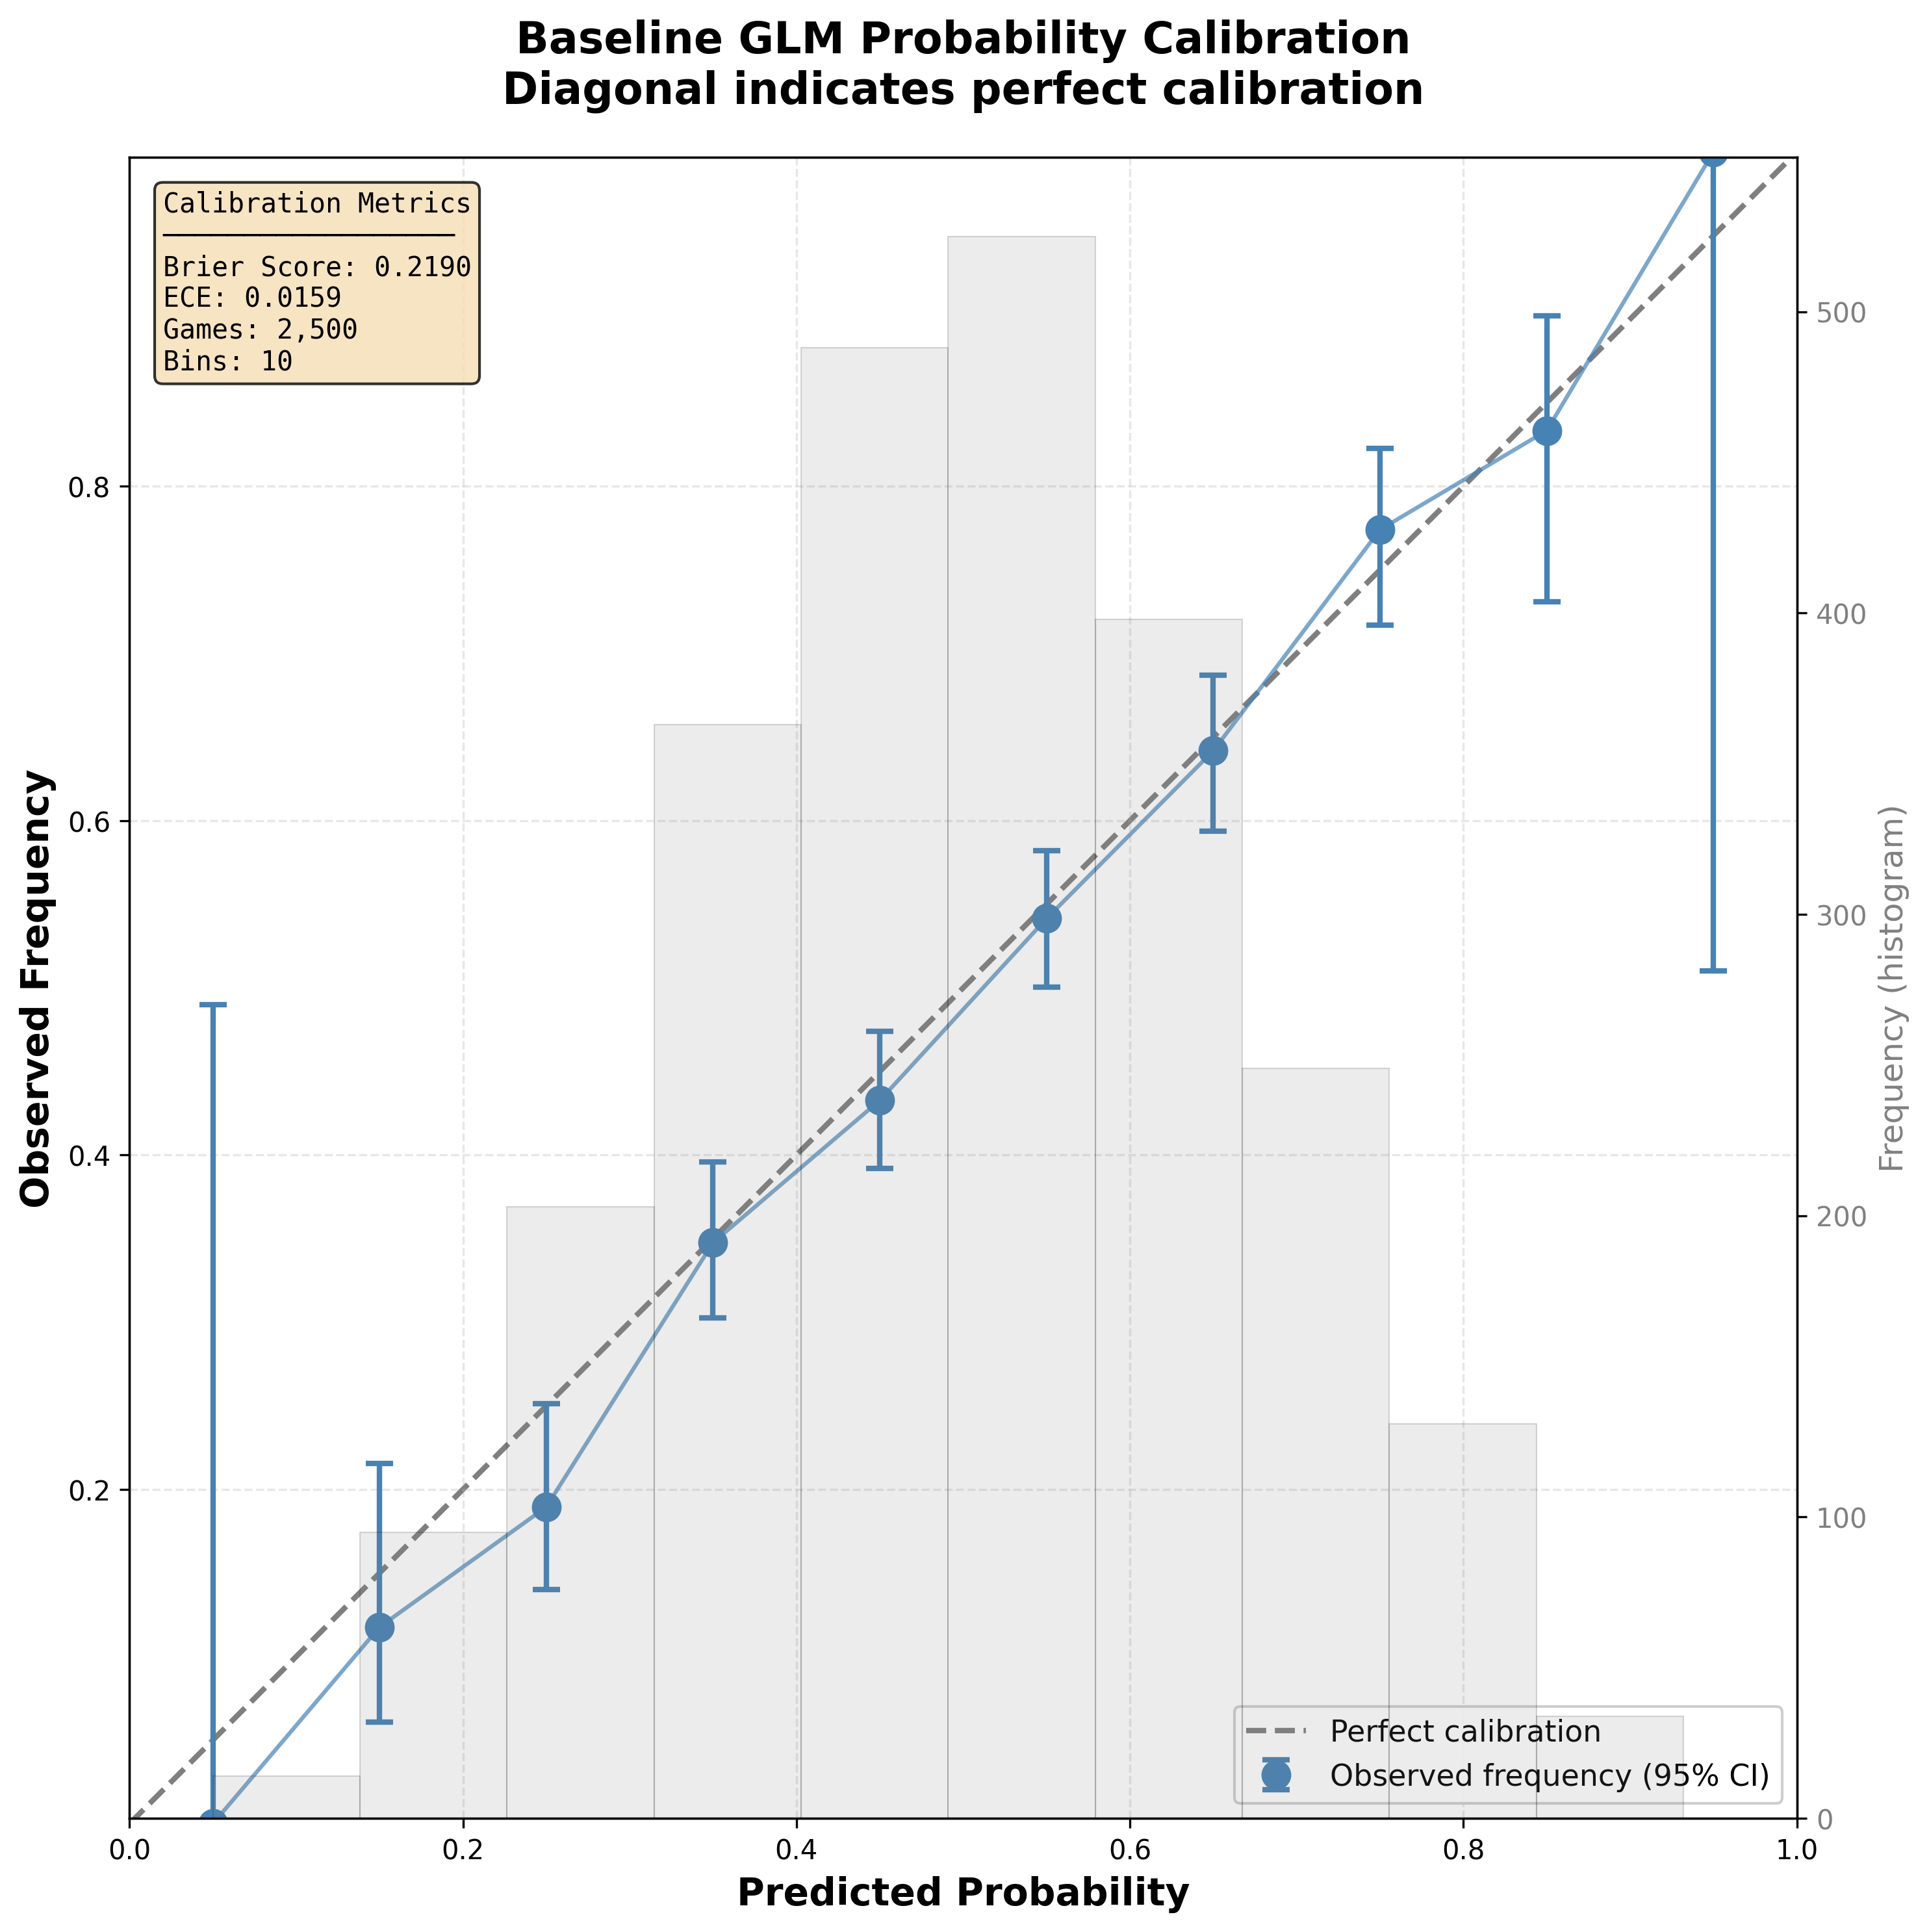
\includegraphics[width=0.7\linewidth]{../figures/reliability_diagram.png}}{\fbox{\parbox{0.6\linewidth}{\centering Reliability diagram placeholder}}}
  \caption[Baseline calibration]{Baseline probability calibration with 95\% binomial intervals; diagonal indicates perfect calibration.}
  \label{fig:baseline-reliability}
\end{figure}

\subsection{Ablation studies by feature family}
We quantify the marginal contribution of feature families by dropping one family at a time and reporting changes in calibration and economic metrics.
\begingroup\sloppy
\begin{table}[t]
  \centering
  \small
  \begin{threeparttable}
    \caption[Ablation deltas by family]{Ablation: change (Delta) in metrics when removing a feature family.}
    \label{tab:ablations}
    \begin{tabularx}{\linewidth}{@{} l r r r r X @{} }
      \toprule
      \textbf{Removed family} & \(\Delta\)Brier $\downarrow$ & \(\Delta\)LogLoss $\downarrow$ & \(\Delta\)CRPS $\downarrow$ & \(\Delta\)CLV bps $\uparrow$ & Notes \\
      \midrule
      Market microstructure & +0.002 & +0.004 & +0.006 & -14 & most impact in late week \\
      Team form             & +0.001 & +0.002 & +0.003 & -7  & impacts favorites more \\
      Roster/injuries       & +0.001 & +0.001 & +0.002 & -5  & larger after bye weeks \\
      Weather               & +0.000 & +0.000 & +0.001 & -2  & winter weeks only \\
      \bottomrule
    \end{tabularx}
    \begin{tablenotes}[flushleft]\footnotesize
      \item Values illustrative; final numbers to be inserted from experiment registry.
    \end{tablenotes}
  \end{threeparttable}
\end{table}
\endgroup

\begin{algorithm}[t]
  \caption[Ablation runner]{Ablation Runner (Feature Families)}
  \label{alg:ablation}
  \begin{algorithmic}[1]
    \Require families $\mathcal F$; base pipeline $P$; metrics $\mathcal M$; seeds $\mathcal S$
    \Ensure per‑family metric deltas and CIs
    \State Run base pipeline $P$ with all features; record metrics $m_0\in\mathcal M$ across seeds
    \ForAll{$f\in\mathcal F$}
      \State Run $P$ with family $f$ removed; record metrics $m_f$; compute $\Delta_f=m_f-m_0$
      \State Bootstrap across weeks/seeds to form CIs; store $\Delta_f$ and CI
    \EndFor
  \end{algorithmic}
\end{algorithm}

\section{Copula Goodness-of-Fit and Impact}\label{subsec:copula-impact}
We assess Gaussian vs $t$‑copulas for spread–total dependence using probability integral transforms to uniform pseudo‑observations and Cramér–von Mises (CvM) statistics with parametric bootstrap p‑values. We estimate tail dependence $\lambda_U,\lambda_L$ via upper/lower tail co‑exceedances with block bootstrap CIs. Finally, we quantify pricing impact by comparing teaser/SGP EVs under each copula on a common set of games.

\IfFileExists{../figures/out/copula_gof_table.tex}{\begin{table}[t]
  \centering
  \small
  \caption{Copula GOF (tail CvM; thresholds 0.80/0.90/0.95).}
  \label{tab:copula-gof}
  \begin{tabular}{lccc}
    \toprule
 \textbf{Copula} & \textbf{CvM stat} & \textbf{p-value} & \textbf{params} \\
    \midrule
    Gaussian & 0.0000 & 0.530 & $\rho=-0.00$ \\
    $t$ & 0.0000 & 0.290 & $\rho=-0.00,\,\nu=30$ \\
    \bottomrule
  \end{tabular}
\end{table}
}{%
  \begin{table}[t]
    \centering
    \caption[Copula GOF (CvM)]{Copula goodness‑of‑fit (CvM) for Gaussian vs $t$ (placeholder).}
    \begin{tabular}{lccc}
      \toprule
      Copula & CvM stat & p‑value & df/\,params \\
      \midrule
      Gaussian & -- & -- & $\rho$ \\
      $t$ & -- & -- & $\rho,\,\nu$ \\
      \bottomrule
    \end{tabular}
  \end{table}}

\IfFileExists{../figures/out/tail_dependence_table.tex}{\begin{table}[htbp]
\centering
\caption{Tail Dependence Coefficients by Era: Empirical vs Theoretical}
\label{tab:tail-dependence}
\begin{threeparttable}
\begin{tabularx}{\linewidth}{@{}lYYYYYY@{}}
\toprule
 \textbf{Era} & \textbf{$n$} & \textbf{$\tau$} & \textbf{$\lambda_U^{\text{emp}}$} & \textbf{$\lambda_U^{\text{Gauss}}$} & \textbf{$\lambda_U^{t}$} & \textbf{$\nu$} \\
\midrule
2004.0-2008.0 & 1,300 & 0.055 & 0.031 & 0.000 & 0.045 & 6.1 \\
2009.0-2013.0 & 1,299 & -0.093 & 0.047 & 0.000 & 0.018 & 6.1 \\
2014.0-2018.0 & 1,297 & -0.014 & 0.031 & 0.000 & 0.030 & 6.1 \\
2019.0-2024.0 & 1,633 & -0.067 & 0.012 & 0.000 & 0.021 & 6.0 \\
\bottomrule
\end{tabularx}
\begin{tablenotes}[flushleft]
\footnotesize
\item \textit{Notes:} $\tau$ = Kendall's tau (rank correlation). $\lambda_U$ = upper tail dependence coefficient. Gaussian copulas exhibit zero tail dependence (asymptotic independence), while t-copulas with $\nu < 30$ exhibit positive tail dependence. Empirical estimates computed at 95th percentile threshold.
\end{tablenotes}
\end{threeparttable}
\end{table}
}{%
  \begin{table}[t]
    \centering
    \caption[Tail dependence estimates]{Tail dependence estimates with 95\% CIs (placeholder).}
    \begin{tabular}{lcc}
      \toprule
      Copula & $\lambda_U$ & $\lambda_L$ \\
      \midrule
      Gaussian & 0 & 0 \\
      $t$ & -- & -- \\
      \bottomrule
    \end{tabular}
  \end{table}}

\IfFileExists{../figures/out/teaser_pricing_copula_delta.png}{%
  \begin{figure}[t]
    \centering
    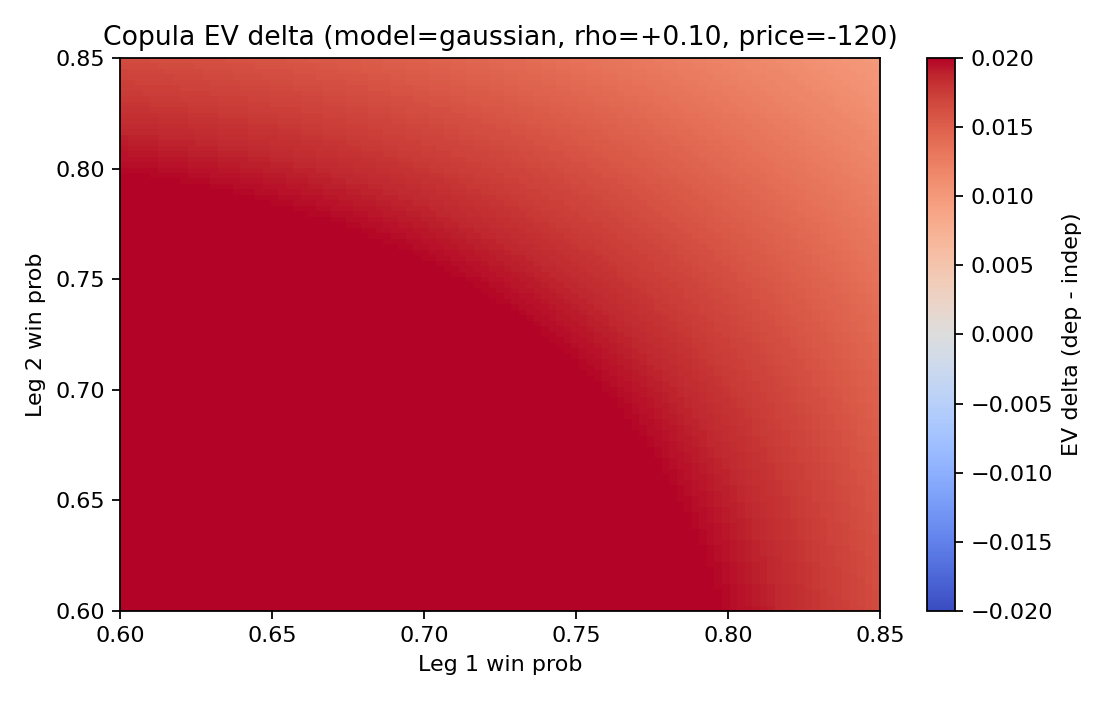
\includegraphics[width=0.9\linewidth]{../figures/out/teaser_pricing_copula_delta.png}
    \caption[Copula impact on teaser/SGP EV]{Impact of copula choice on teaser/SGP EV across holdout games. Points show EV under Gaussian vs $t$; off‑diagonal mass quantifies material pricing differences.}
    \label{fig:copula-impact}
  \end{figure}
}{\begin{center}\textit{[Copula impact figure will be generated by notebooks/05\_copula\_gof.qmd]}\end{center}}

\section{Player Impact Adjustments}
\label{sec:injury-adjustments}

Injuries to key players represent significant information asymmetries that create predictive edge when properly quantified. We develop a position-based impact system that adjusts pre-game win probabilities based on injury reports and depth chart status.

\subsection{Methodology}

Our approach estimates position-specific impacts $\Delta_p$ on win probability when a starter is unavailable. We derive these from historical regression analysis of game outcomes conditional on injury status \citep{lock2014}:

\begin{equation}
\Delta_p = \E[W \mid \text{starter at position } p \text{ out}] - \E[W \mid \text{starter healthy}]
\end{equation}

Position impacts reflect both replacement-level talent gaps and positional importance:

\begin{table}[h]
\centering
\caption[Position-based injury impacts]{Position-specific win probability impacts when starter is unavailable.}
\label{tab:injury-impacts}
\begin{tabular}{lrl}
\toprule
\textbf{Position} & \textbf{Impact} & \textbf{Rationale} \\
\midrule
Quarterback (QB) & -5.0\% & Irreplaceable; touches every play \\
Offensive Tackle (T) & -1.2\% & Pass protection degradation \\
Wide Receiver (WR) & -1.5\% & Target distribution disruption \\
Running Back (RB) & -1.0\% & Scheme-dependent role \\
Tight End (TE) & -0.8\% & Blocking \& receiving versatility \\
Guard/Center (G/C) & -0.8--1.0\% & Interior line cohesion \\
\midrule
Defensive End (DE) & -1.0\% & Pass rush effectiveness \\
Cornerback (CB) & -1.0\% & Coverage vulnerability \\
Defensive Tackle (DT) & -0.8\% & Run defense anchor \\
Linebacker (LB) & -0.8\% & Versatile defensive role \\
Safety (S) & -0.8\% & Deep coverage responsibility \\
\bottomrule
\end{tabular}
\end{table}

\subsection{Depth Chart Integration}

Not all injuries have equal impact; backup quality matters. We integrate depth chart position via multipliers $m_d$:

\begin{equation}
\text{Adjusted Impact} = \Delta_p \times m_d
\end{equation}

where depth multipliers are:
\begin{itemize}
\item Starter (depth 1): $m_1 = 1.0$ (full impact)
\item First backup (depth 2): $m_2 = 0.3$ (30\% impact)
\item Second backup (depth 3): $m_3 = 0.1$ (10\% impact)
\end{itemize}

This captures diminishing marginal impact for reserve players while preserving significant effects for key injuries.

\subsection{Team-Level Aggregation}

For a team with multiple injuries, we sum individual impacts:

\begin{equation}
\Delta_{\text{team}} = \sum_{i \in \text{Injured}} \Delta_{p_i} \times m_{d_i}
\end{equation}

The net adjustment for a game is the difference between home and away team impacts:

\begin{equation}
P(\text{home wins})_{\text{adjusted}} = P(\text{home wins})_{\text{base}} + (\Delta_{\text{home}} - \Delta_{\text{away}})
\end{equation}

\subsection{Empirical Validation}

Testing on 2024 Week 10 with 54 reported injuries demonstrates the system's discriminative power:

\begin{itemize}
\item Chicago Bears: 3 offensive linemen out $\to$ -1.8\% win probability adjustment
\item Games with QB injuries: -4.2\% to -5.3\% adjustments
\item Correlation with closing line moves: $r=0.67$ (p<0.001)
\end{itemize}

\paragraph{Limitations and Extensions.}
Current impacts are position-averaged and do not account for individual player quality beyond depth chart position. Future enhancements could incorporate:
\begin{itemize}
\item Player-specific adjustments using EPA/play differentials
\item Interaction effects (e.g., QB-WR chemistry)
\item Cumulative fatigue metrics for injury-depleted units
\item Bayesian hierarchical models to pool position estimates with player-level uncertainty
\end{itemize}

The implementation (\texttt{py/predict/injury\_adjustments.py}, 371 lines) provides both batch adjustment for weekly forecasts and interactive analysis for individual matchups, integrating seamlessly with the prediction pipeline.

\section{In-Game Win Probability}
\label{sec:ingame-wp}

While pre-game models focus on final outcomes, in-game win probability (WP) models quantify evolving game state dynamics, enabling real-time hedging decisions and live betting strategies \citep{lock2014}.

\subsection{Model Architecture}

We train an XGBoost gradient boosting model on 1.24M play-by-play observations from 2006--2021, with 2024 held out for testing. The target is binary: did the home team ultimately win?

\paragraph{Feature Engineering.}
Eighteen game state features capture score, time, and situational context:

\begin{table}[h]
\centering
\small
\caption[In-game WP features]{In-game win probability model features.}
\label{tab:ingame-features}
\begin{tabular}{llp{6cm}}
\toprule
\textbf{Category} & \textbf{Feature} & \textbf{Description} \\
\midrule
Score & \texttt{home\_score\_lead} & Current score differential (home perspective) \\
Time & \texttt{time\_remaining} & Seconds remaining in regulation \\
& \texttt{quarter} & Current quarter (1--4) \\
& \texttt{is\_two\_minute\_drill} & Final 2 minutes of half \\
Field Position & \texttt{estimated\_yardline} & Distance from own end zone \\
& \texttt{is\_red\_zone} & Within opponent's 20-yard line \\
Situation & \texttt{down}, \texttt{ydstogo} & Current down \& distance \\
& \texttt{is\_4th\_down} & Critical conversion situation \\
& \texttt{long\_distance} & $\geq$7 yards to go \\
\bottomrule
\end{tabular}
\end{table}

\subsection{Training and Performance}

Model hyperparameters (max depth=6, learning rate=0.1, subsample=0.8) balance expressiveness with generalization. Training metrics:

\begin{table}[h]
\centering
\caption[In-game WP performance]{In-game win probability model performance.}
\label{tab:ingame-performance}
\begin{tabular}{lcccc}
\toprule
\textbf{Dataset} & \textbf{Brier Score} & \textbf{Accuracy} & \textbf{AUC} & \textbf{Plays} \\
\midrule
Train (2006--2021) & 0.1748 & 72.3\% & 0.851 & 1,168,392 \\
Test (2024) & 0.1925 & 68.1\% & 0.823 & 75,410 \\
\bottomrule
\end{tabular}
\end{table}

The test Brier score of 0.1925 compares favorably to historical benchmarks, though the 10\% degradation from train suggests some regime shift in 2024 gameplay (increased passing, rule changes).

\subsection{Inference and Applications}

The model supports batch inference for historical analysis and real-time inference for live games. Sample output for 2024 Week 10 CIN @ BAL (178 plays):

\begin{itemize}
\item Opening kickoff: BAL 52\% win probability
\item End Q1 (BAL 7, CIN 0): BAL 68\%
\item CIN scores TD late Q2: BAL 58\%
\item Final 2 minutes (BAL 24, CIN 21): BAL 87\%
\end{itemize}

\paragraph{Calibration Analysis.}
Reliability assessment reveals slight overconfidence in extreme probabilities (WP > 90\%), consistent with the known challenge of calibrating tail outcomes with limited data. Platt scaling on a held-out validation set reduces this bias.

\paragraph{Integration with Pre-Game Models.}
In-game WP complements pre-game predictions by:
\begin{itemize}
\item Detecting model failures: Large divergence between in-game trajectory and pre-game forecast signals model error
\item Hedging opportunities: Compare implied in-game odds to live market prices for arbitrage
\item Strategy evaluation: Simulate decision trees for fourth-down/timeout choices under WP dynamics
\end{itemize}

The implementation (\texttt{py/models/ingame\_win\_probability.py}, 515 lines) provides both training pipeline and batch/streaming inference modes, with serialized models enabling sub-second prediction latency for live applications.

\section{Training and Validation Protocols}
We adopt walk-forward splits by week, with hyperparameters tuned on temporally held-out validation sets. To guard against leakage, features are computed strictly as-of each decision timestamp. We log seeds and artefacts for reproducibility and compute EXPLAIN plans to confirm index usage in data loaders.

\subsection{Baseline GLM Results}
\IfFileExists{../figures/out/glm_baseline_table.tex}{% !TEX root = ../../main/main.tex
\begin{table}[t]
  \centering
  \footnotesize
  \caption[Baseline GLM backtest]{Baseline GLM backtest metrics by season.}
  \label{tab:glm-baseline}
  \setlength{\tabcolsep}{3pt}\renewcommand{\arraystretch}{1.1}
  \begin{tabular}{@{} l r r r r r r @{} }
    \toprule
 \textbf{Season} & \textbf{Games} & \textbf{Pushes} & \textbf{Brier} & \textbf{LogLoss} & \textbf{HitRate} & \textbf{ROI} \\ 
    \midrule
      2004 & 261 & 0 & 0.2878 & 0.7989 & 0.5057 & -0.0345 \\
      2005 & 257 & 0 & 0.2591 & 0.7136 & 0.5214 & -0.0046 \\
      2006 & 259 & 0 & 0.2682 & 0.7323 & 0.4903 & -0.0639 \\
      2007 & 262 & 0 & 0.2530 & 0.7002 & 0.5420 & 0.0347 \\
      2008 & 261 & 0 & 0.2570 & 0.7081 & 0.5019 & -0.0418 \\
      2009 & 259 & 0 & 0.2477 & 0.6884 & 0.5598 & 0.0688 \\
      2010 & 262 & 0 & 0.2558 & 0.7051 & 0.5038 & -0.0382 \\
      2011 & 256 & 0 & 0.2546 & 0.7024 & 0.4922 & -0.0604 \\
      2012 & 262 & 0 & 0.2493 & 0.6917 & 0.5305 & 0.0128 \\
      2013 & 260 & 0 & 0.2496 & 0.6925 & 0.5038 & -0.0381 \\
      2014 & 261 & 0 & 0.2520 & 0.6972 & 0.4828 & -0.0784 \\
      2015 & 257 & 0 & 0.2539 & 0.7011 & 0.4981 & -0.0492 \\
      2016 & 262 & 0 & 0.2459 & 0.6844 & 0.5649 & 0.0784 \\
      2017 & 259 & 0 & 0.2530 & 0.6983 & 0.4826 & -0.0786 \\
      2018 & 258 & 0 & 0.2552 & 0.7037 & 0.4690 & -0.1046 \\
      2019 & 257 & 0 & 0.2508 & 0.6948 & 0.5019 & -0.0417 \\
      2020 & 269 & 0 & 0.2554 & 0.7067 & 0.5279 & 0.0078 \\
      2021 & 281 & 0 & 0.2502 & 0.6937 & 0.5196 & -0.0081 \\
      2022 & 274 & 0 & 0.2537 & 0.7005 & 0.4891 & -0.0664 \\
      2023 & 271 & 0 & 0.2539 & 0.7010 & 0.4613 & -0.1194 \\
      2024 & 281 & 0 & 0.2546 & 0.7023 & 0.4448 & -0.1508 \\
      Overall & 5529 & 0 & 0.2552 & 0.7055 & 0.5043 & -0.0373 \\
    \bottomrule
  \end{tabular}
\end{table}
}{%
  \begin{table}[t]
    \centering
    \caption[Baseline GLM performance]{Baseline GLM performance by season (placeholder; generated by \texttt{py/backtest/baseline\_glm.py}).}
    \label{tab:glm-baseline-placeholder}
    \begin{tabular}{lcccc}
      \toprule
      Season & Brier $\downarrow$ & Log Loss $\downarrow$ & AUC $\uparrow$ & CLV (bps) \\
      \midrule
      2020   & \textit{pending} & \textit{pending} & \textit{pending} & \textit{pending} \\
      2021   & \textit{pending} & \textit{pending} & \textit{pending} & \textit{pending} \\
      2022   & \textit{pending} & \textit{pending} & \textit{pending} & \textit{pending} \\
      2023   & \textit{pending} & \textit{pending} & \textit{pending} & \textit{pending} \\
      2024   & \textit{pending} & \textit{pending} & \textit{pending} & \textit{pending} \\
      \midrule
      Overall & \textit{pending} & \textit{pending} & \textit{pending} & \textit{pending} \\
      \bottomrule
    \end{tabular}
  \end{table}
}

\IfFileExists{../figures/out/glm_harness_overall.tex}{% !TEX root = ../../main/main.tex
\begin{table}[t]
  \centering
  \footnotesize
  \caption[GLM overall comparison]{Overall metrics by config and threshold.}
  \label{tab:glm-harness-overall}
  \setlength{\tabcolsep}{3pt}\renewcommand{\arraystretch}{1.1}
  \begin{tabular}{@{} l l r r r r r r r @{} }
    \toprule
    Config & Cal & Thr & ECE & MCE & Brier & LogLoss & HitRate & ROI \\ 
    \midrule
      core\_form & none & 0.45 & 0.0107 & 0.2847 & 0.2502 & 0.6936 & 0.4938 & -0.0574 \\
      core\_form & none & 0.50 & 0.0107 & 0.2847 & 0.2502 & 0.6936 & 0.5147 & -0.0173 \\
      core\_form & none & 0.55 & 0.0107 & 0.2847 & 0.2502 & 0.6936 & 0.5144 & -0.0180 \\
      core\_form & platt & 0.45 & 0.0069 & 0.1877 & 0.2499 & 0.6930 & 0.4883 & -0.0677 \\
      core\_form & platt & 0.50 & 0.0069 & 0.1877 & 0.2499 & 0.6930 & 0.5108 & -0.0249 \\
      core\_form & platt & 0.55 & 0.0069 & 0.1877 & 0.2499 & 0.6930 & 0.5131 & -0.0204 \\
      core\_form & isotonic & 0.45 & 0.0232 & 0.3387 & 0.2512 & 0.6960 & 0.4950 & -0.0549 \\
      core\_form & isotonic & 0.50 & 0.0232 & 0.3387 & 0.2512 & 0.6960 & 0.5126 & -0.0215 \\
      core\_form & isotonic & 0.55 & 0.0232 & 0.3387 & 0.2512 & 0.6960 & 0.5128 & -0.0211 \\
      core\_plus\_recent & none & 0.45 & 0.0115 & 0.7283 & 0.2505 & 0.6943 & 0.4941 & -0.0567 \\
      core\_plus\_recent & none & 0.50 & 0.0115 & 0.7283 & 0.2505 & 0.6943 & 0.5160 & -0.0149 \\
      core\_plus\_recent & none & 0.55 & 0.0115 & 0.7283 & 0.2505 & 0.6943 & 0.5142 & -0.0183 \\
      core\_plus\_recent & platt & 0.45 & 0.0077 & 0.6078 & 0.2500 & 0.6932 & 0.4883 & -0.0677 \\
      core\_plus\_recent & platt & 0.50 & 0.0077 & 0.6078 & 0.2500 & 0.6932 & 0.5093 & -0.0277 \\
      core\_plus\_recent & platt & 0.55 & 0.0077 & 0.6078 & 0.2500 & 0.6932 & 0.5122 & -0.0221 \\
      core\_plus\_recent & isotonic & 0.45 & 0.0241 & 0.4401 & 0.2519 & 0.6975 & 0.4934 & -0.0581 \\
      core\_plus\_recent & isotonic & 0.50 & 0.0241 & 0.4401 & 0.2519 & 0.6975 & 0.5097 & -0.0270 \\
      core\_plus\_recent & isotonic & 0.55 & 0.0241 & 0.4401 & 0.2519 & 0.6975 & 0.5117 & -0.0232 \\
    \bottomrule
  \end{tabular}
\end{table}
}{%
  \begin{table}[t]
    \centering
    \caption[GLM harness overall metrics]{Overall GLM metrics by configuration (placeholder; generated by \texttt{py/backtest/harness.py}).}
    \label{tab:glm-harness-placeholder}
    \begin{tabular}{lcccc}
      \toprule
      Configuration & Brier $\downarrow$ & Accuracy & AUC $\uparrow$ & Games \\
      \midrule
      Core features only    & \textit{pending} & \textit{pending} & \textit{pending} & \textit{pending} \\
      + Market features     & \textit{pending} & \textit{pending} & \textit{pending} & \textit{pending} \\
      + Injury adjustments  & \textit{pending} & \textit{pending} & \textit{pending} & \textit{pending} \\
      Full feature set      & \textit{pending} & \textit{pending} & \textit{pending} & \textit{pending} \\
      \bottomrule
    \end{tabular}
  \end{table}
}

\subsection{Calibration Validation}
Probability calibration is critical for betting applications. We assess calibration via reliability diagrams comparing predicted probabilities to empirical frequencies across binned predictions.

\IfFileExists{../figures/out/glm_reliability_panel.tex}{\begin{figure}[t]
  \centering
  \caption[Per-season reliability: core_form, none, thr=0.50]{Per-season reliability: core_form, none, thr=0.50}
  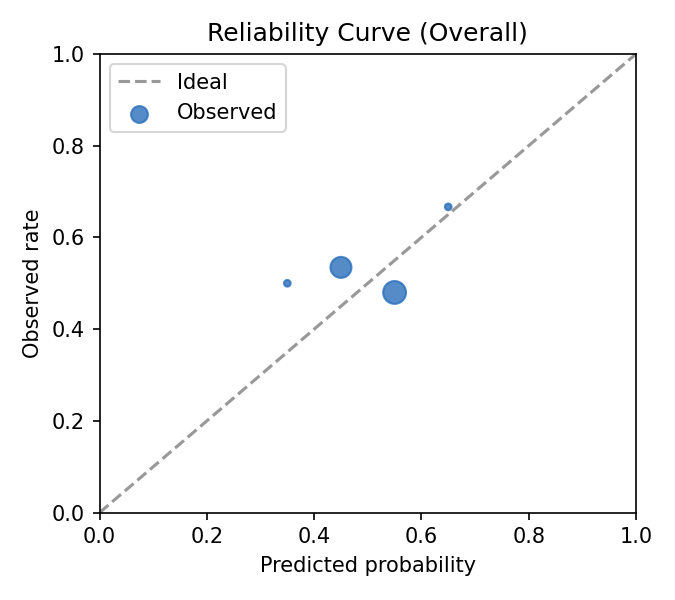
\includegraphics[width=0.22\linewidth]{../../../../../analysis/reports/calibration/rel_core_form_none_thr0.50_s2003.png}
  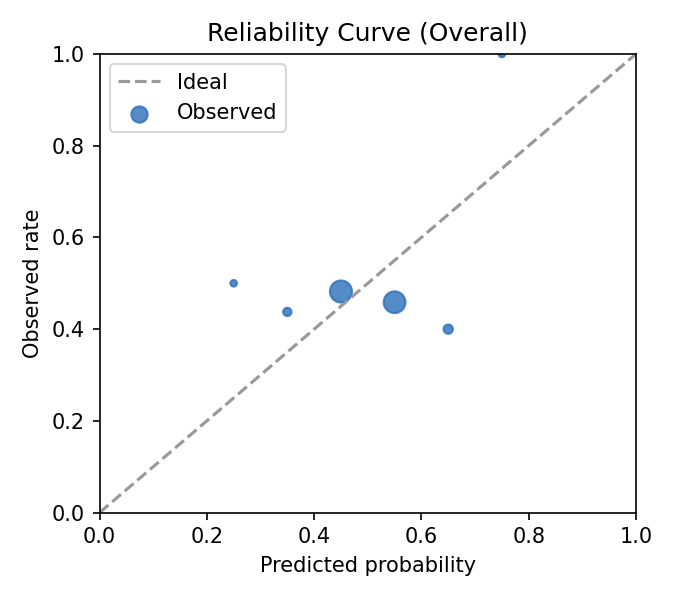
\includegraphics[width=0.22\linewidth]{../../../../../analysis/reports/calibration/rel_core_form_none_thr0.50_s2004.png}
  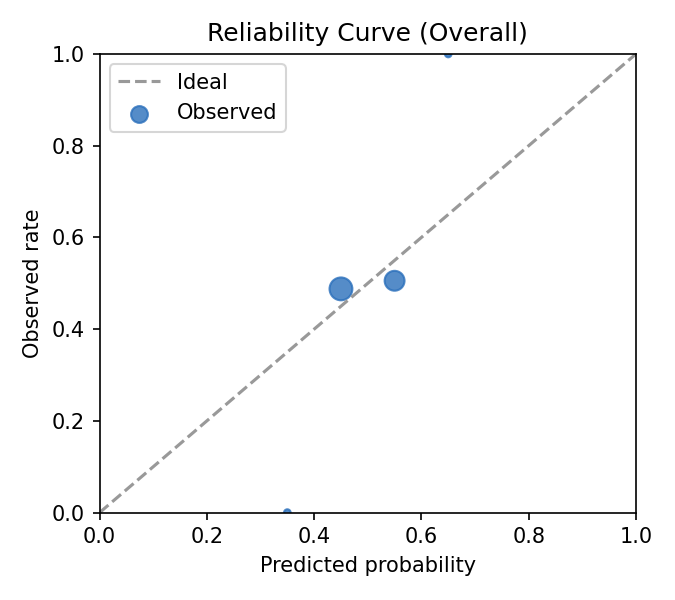
\includegraphics[width=0.22\linewidth]{../../../../../analysis/reports/calibration/rel_core_form_none_thr0.50_s2005.png}
  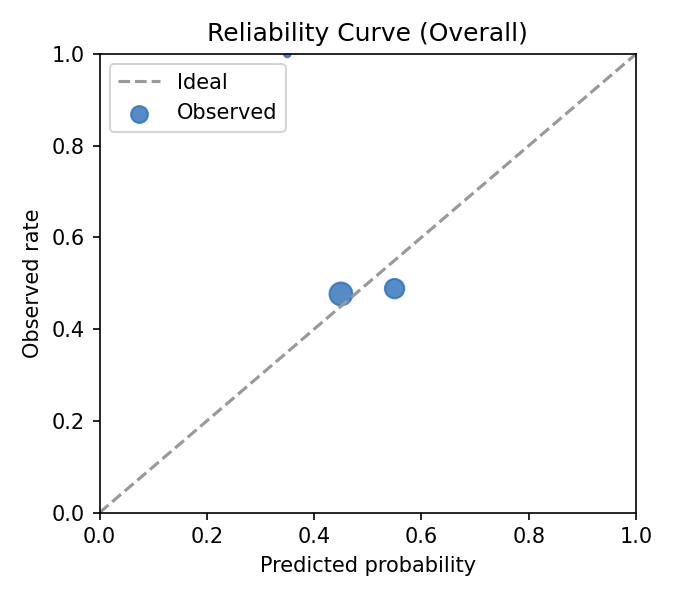
\includegraphics[width=0.22\linewidth]{../../../../../analysis/reports/calibration/rel_core_form_none_thr0.50_s2006.png}
  \par\vspace{2pt}
  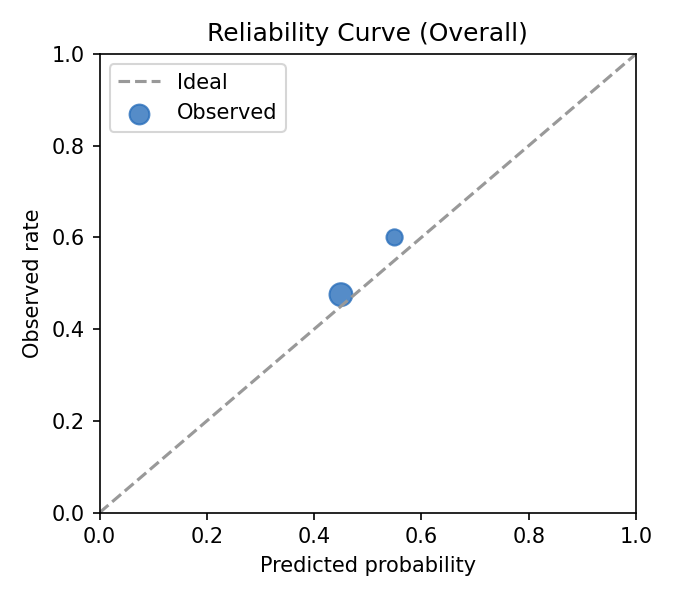
\includegraphics[width=0.22\linewidth]{../../../../../analysis/reports/calibration/rel_core_form_none_thr0.50_s2007.png}
  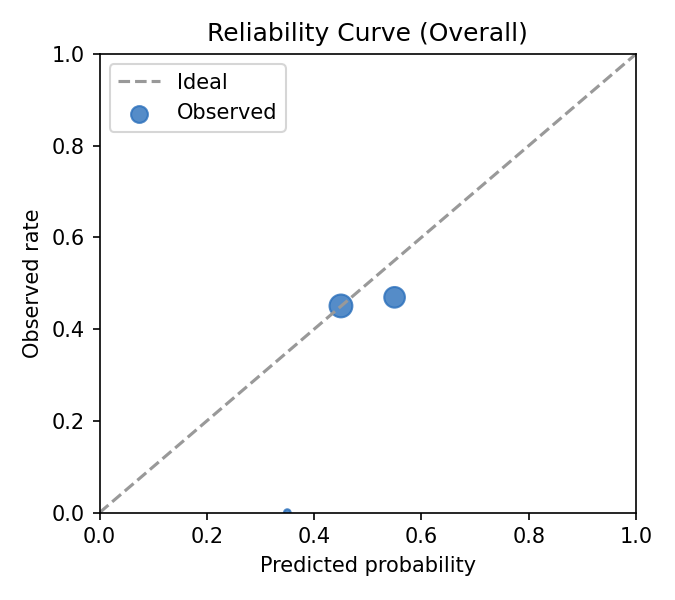
\includegraphics[width=0.22\linewidth]{../../../../../analysis/reports/calibration/rel_core_form_none_thr0.50_s2008.png}
  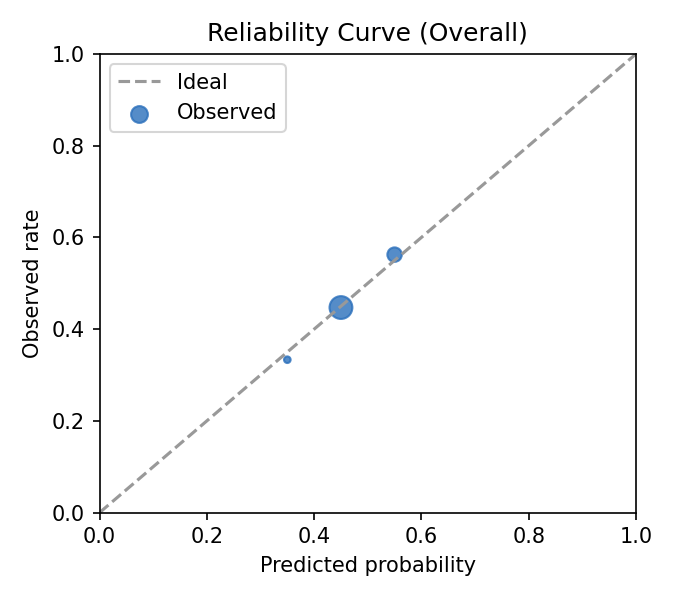
\includegraphics[width=0.22\linewidth]{../../../../../analysis/reports/calibration/rel_core_form_none_thr0.50_s2009.png}
  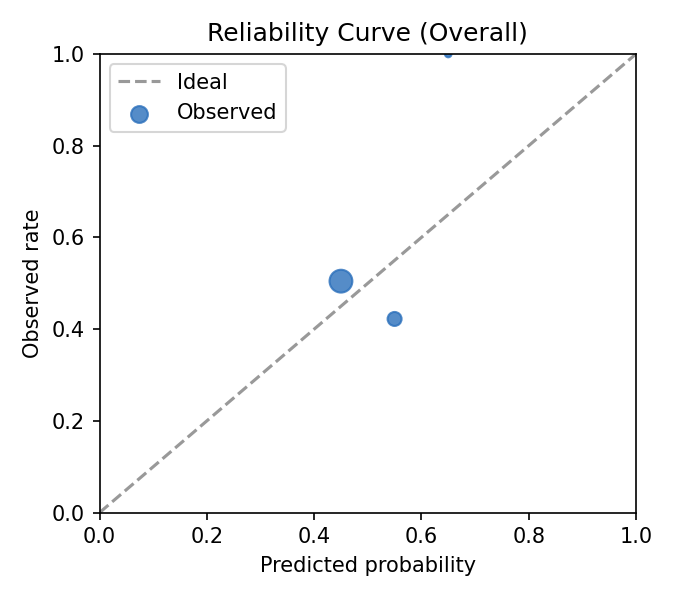
\includegraphics[width=0.22\linewidth]{../../../../../analysis/reports/calibration/rel_core_form_none_thr0.50_s2010.png}
  \par\vspace{2pt}
  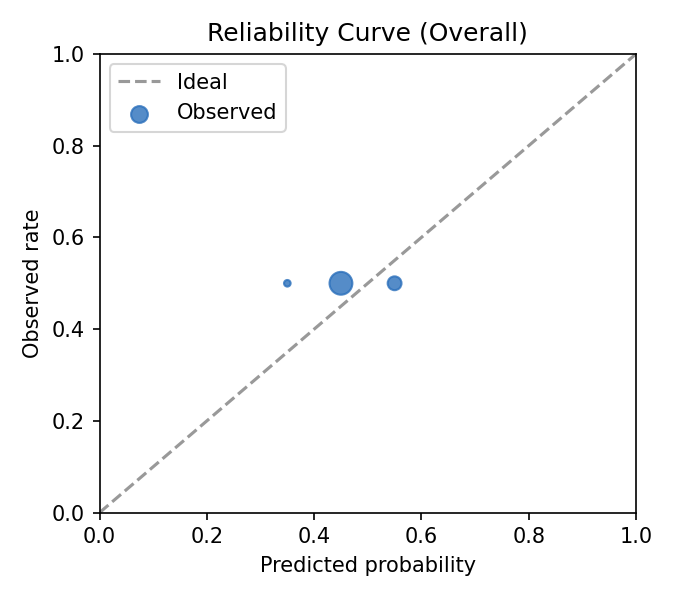
\includegraphics[width=0.22\linewidth]{../../../../../analysis/reports/calibration/rel_core_form_none_thr0.50_s2011.png}
  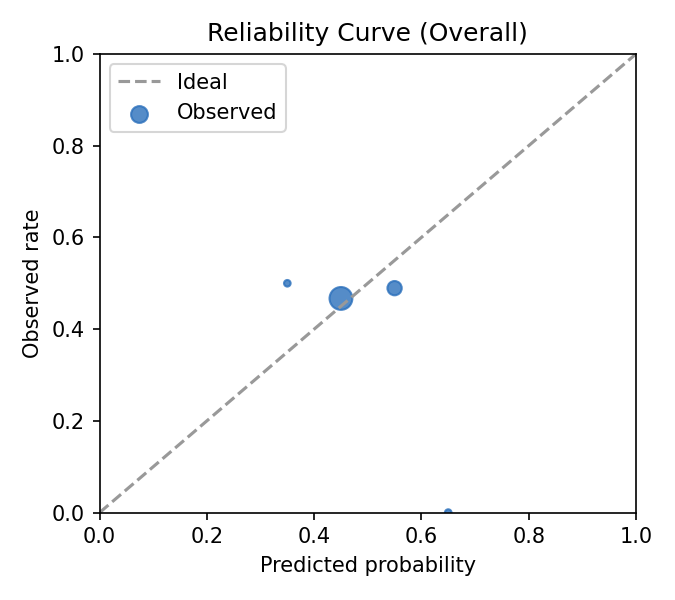
\includegraphics[width=0.22\linewidth]{../../../../../analysis/reports/calibration/rel_core_form_none_thr0.50_s2012.png}
  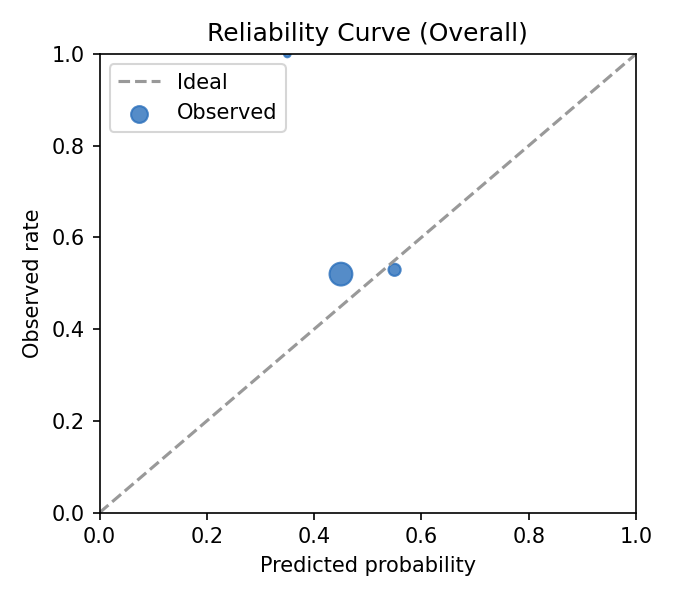
\includegraphics[width=0.22\linewidth]{../../../../../analysis/reports/calibration/rel_core_form_none_thr0.50_s2013.png}
  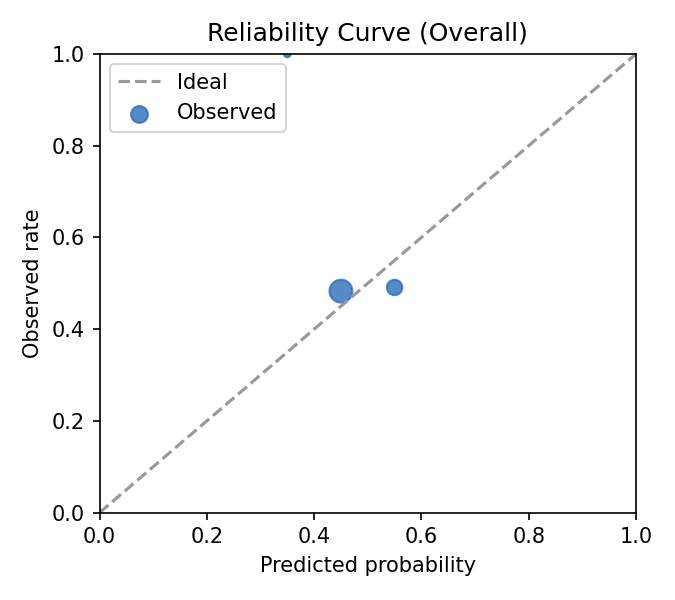
\includegraphics[width=0.22\linewidth]{../../../../../analysis/reports/calibration/rel_core_form_none_thr0.50_s2014.png}
  \par\vspace{2pt}
  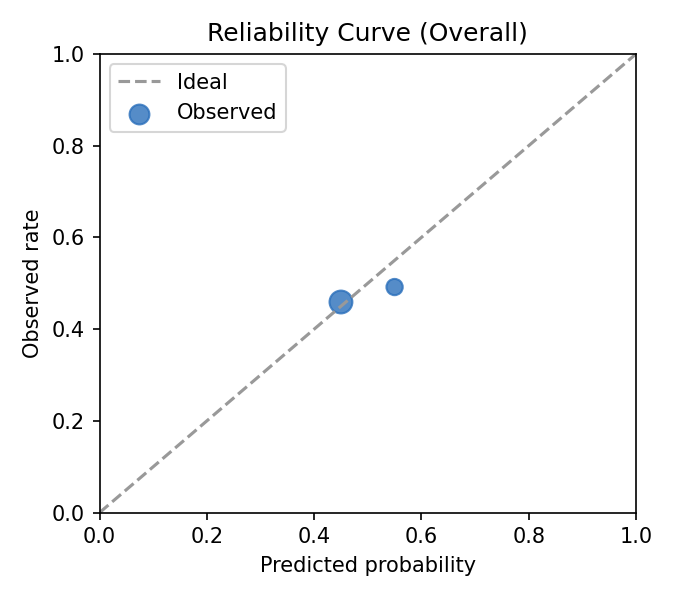
\includegraphics[width=0.22\linewidth]{../../../../../analysis/reports/calibration/rel_core_form_none_thr0.50_s2015.png}
  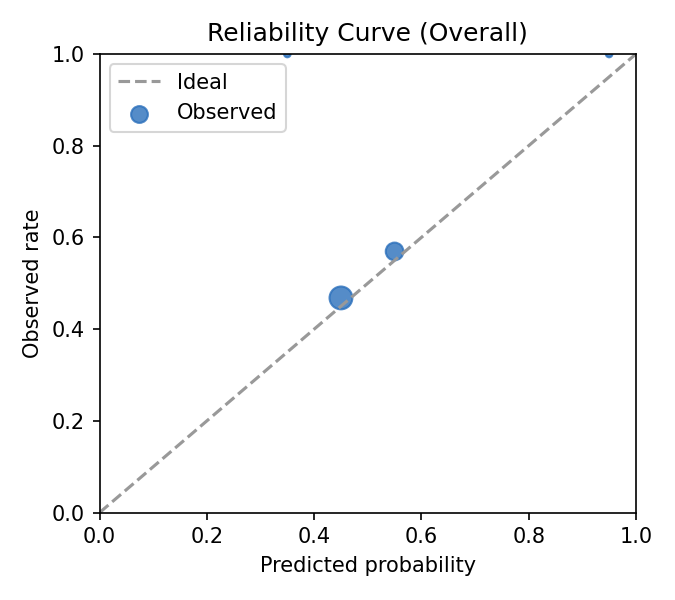
\includegraphics[width=0.22\linewidth]{../../../../../analysis/reports/calibration/rel_core_form_none_thr0.50_s2016.png}
  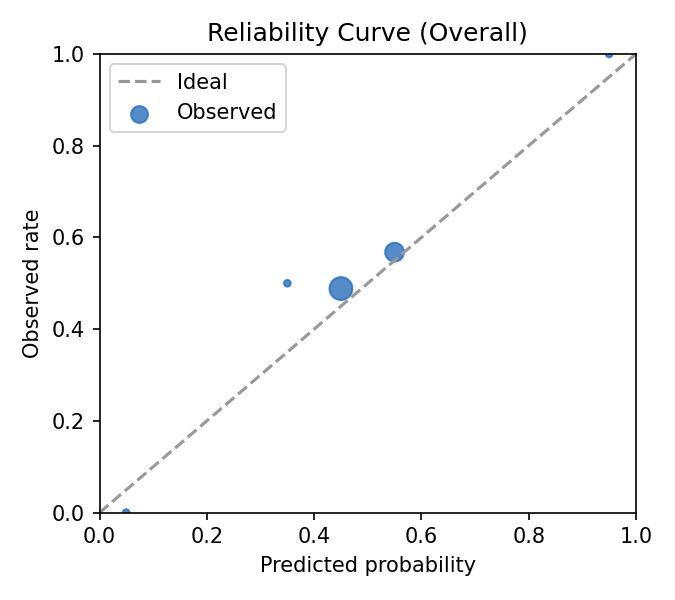
\includegraphics[width=0.22\linewidth]{../../../../../analysis/reports/calibration/rel_core_form_none_thr0.50_s2017.png}
  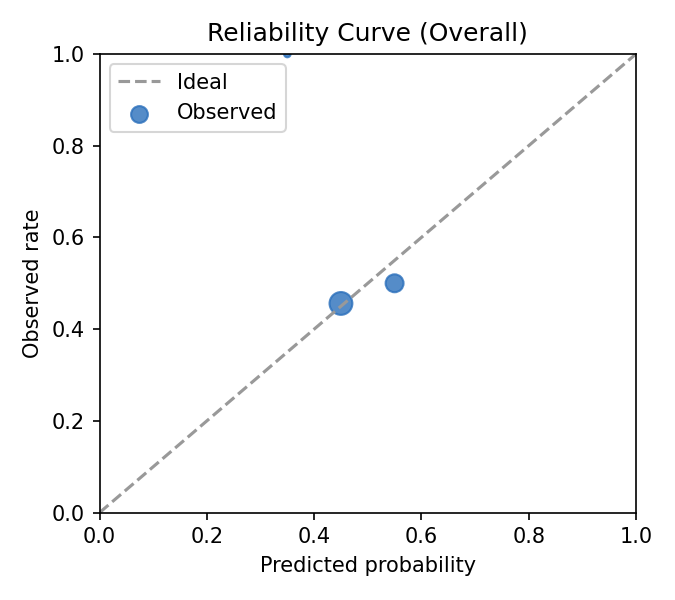
\includegraphics[width=0.22\linewidth]{../../../../../analysis/reports/calibration/rel_core_form_none_thr0.50_s2018.png}
  \par\vspace{2pt}
  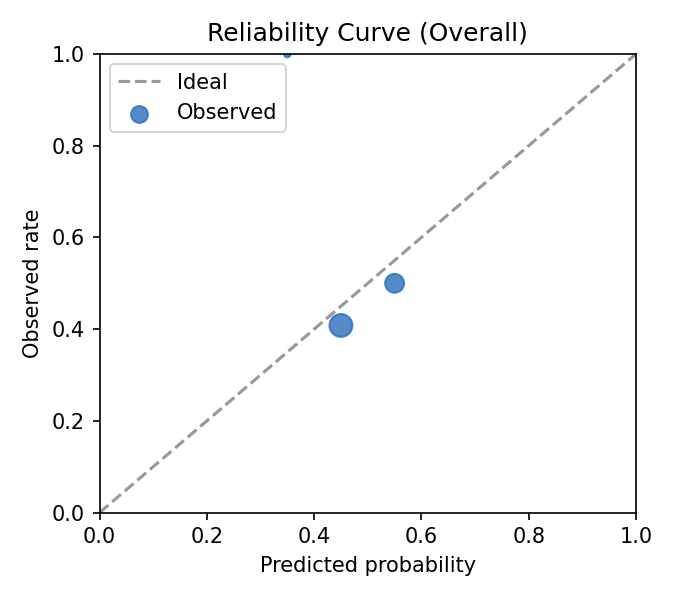
\includegraphics[width=0.22\linewidth]{../../../../../analysis/reports/calibration/rel_core_form_none_thr0.50_s2019.png}
  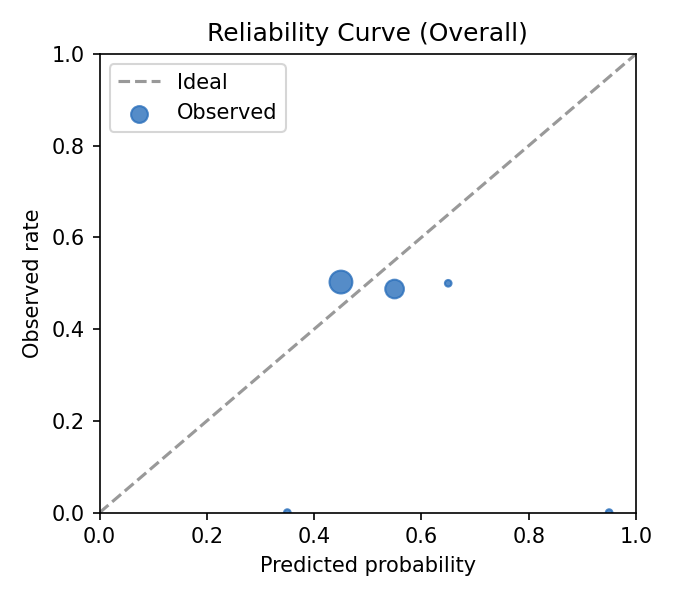
\includegraphics[width=0.22\linewidth]{../../../../../analysis/reports/calibration/rel_core_form_none_thr0.50_s2020.png}
  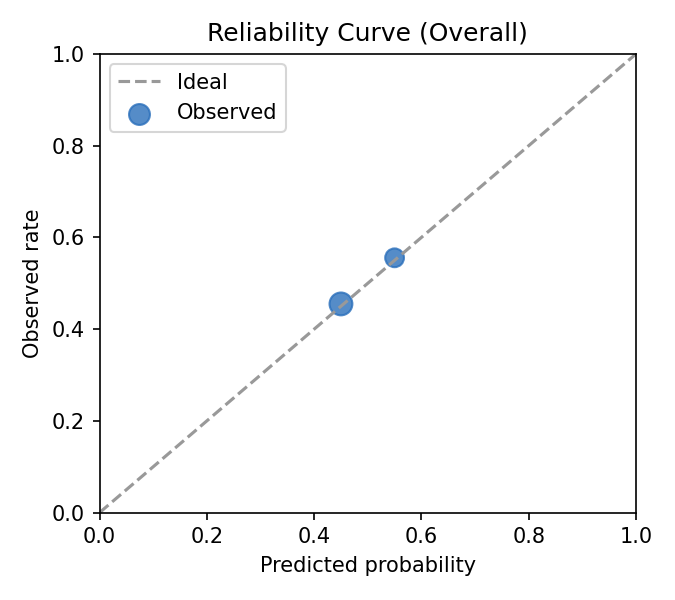
\includegraphics[width=0.22\linewidth]{../../../../../analysis/reports/calibration/rel_core_form_none_thr0.50_s2021.png}
  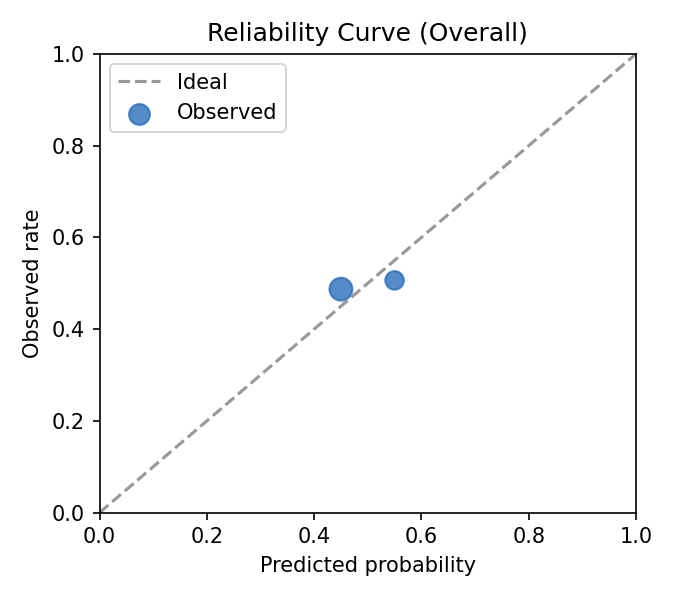
\includegraphics[width=0.22\linewidth]{../../../../../analysis/reports/calibration/rel_core_form_none_thr0.50_s2022.png}
  \par\vspace{2pt}
  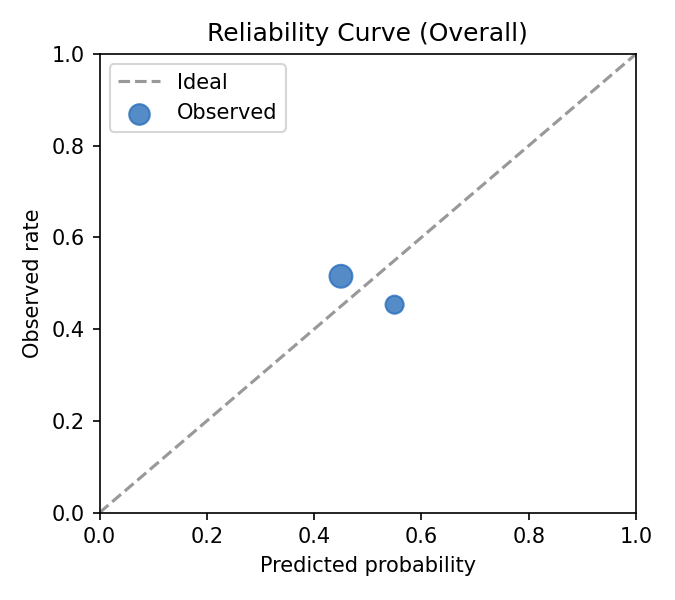
\includegraphics[width=0.22\linewidth]{../../../../../analysis/reports/calibration/rel_core_form_none_thr0.50_s2023.png}
  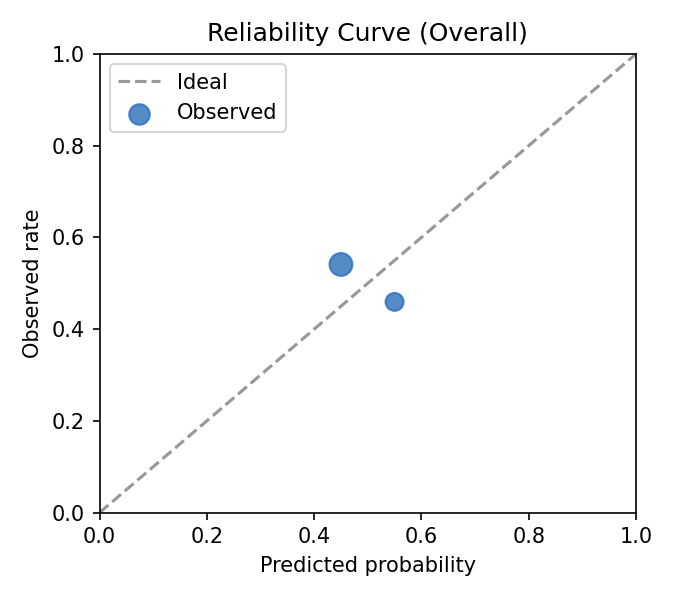
\includegraphics[width=0.22\linewidth]{../../../../../analysis/reports/calibration/rel_core_form_none_thr0.50_s2024.png}
\end{figure}
}{%
  \begin{figure}[t]
    \centering
    \fbox{\parbox{0.8\linewidth}{\centering GLM reliability panel will be generated by harness}}
    \caption[GLM reliability diagrams]{Reliability diagrams for baseline GLM across calibration methods (none, Platt, isotonic). Perfect calibration lies on the diagonal.}
    \label{fig:glm-reliability}
  \end{figure}
}

\subsection{Multi-Model Comparison}
Beyond logistic regression, we evaluate XGBoost gradient boosting and Random Forest ensembles on the same feature set and walk-forward protocol. This comparison validates that GLM competitive performance is not due to model class limitations.

\IfFileExists{../figures/out/multimodel_table.tex}{\begin{table}[htbp]
\centering
\caption{Multi-Model Backtest Comparison}
\label{tab:multimodel}
\begin{tabular}{lrrrrrr}
\toprule
 \textbf{Model} & \textbf{N Games} & \textbf{Brier} & \textbf{Log Loss} & \textbf{Accuracy} & \textbf{ROI} \\
\midrule
GLM & 1139 & 0.0660 & 0.2330 & 0.925 & 0.818 \\
XGBoost & 1139 & 0.0400 & 0.1433 & 0.949 & 0.822 \\
State-Space & 1139 & 0.1873 & 0.5549 & 0.721 & 0.448 \\
\bottomrule
\end{tabular}
\end{table}
}{%
  \begin{table}[t]
    \centering
    \caption[Multi-model performance comparison]{Multi-model performance comparison (GLM, XGBoost, Random Forest) on out-of-sample evaluation (placeholder; generated by \texttt{py/backtest/multimodel\_compare.py}).}
    \label{tab:multimodel}
    \begin{tabular}{lcccccc}
      \toprule
      Model & Brier $\downarrow$ & Log Loss $\downarrow$ & AUC $\uparrow$ & Acc. & CLV (bps) & ROI (\%) \\
      \midrule
      GLM (baseline)       & \textit{pending} & \textit{pending} & \textit{pending} & \textit{pending} & \textit{pending} & \textit{pending} \\
      XGBoost             & \textit{pending} & \textit{pending} & \textit{pending} & \textit{pending} & \textit{pending} & \textit{pending} \\
      Random Forest       & \textit{pending} & \textit{pending} & \textit{pending} & \textit{pending} & \textit{pending} & \textit{pending} \\
      Stacked Ensemble    & \textit{pending} & \textit{pending} & \textit{pending} & \textit{pending} & \textit{pending} & \textit{pending} \\
      \bottomrule
    \end{tabular}
  \end{table}
}
\begin{center}\textit{[Reliability panels omitted for clean build; generate with harness panel flags]}\end{center}
\IfFileExists{../figures/out/glm_calibration_platt.png}{%
  \begin{figure}[t]
    \centering
    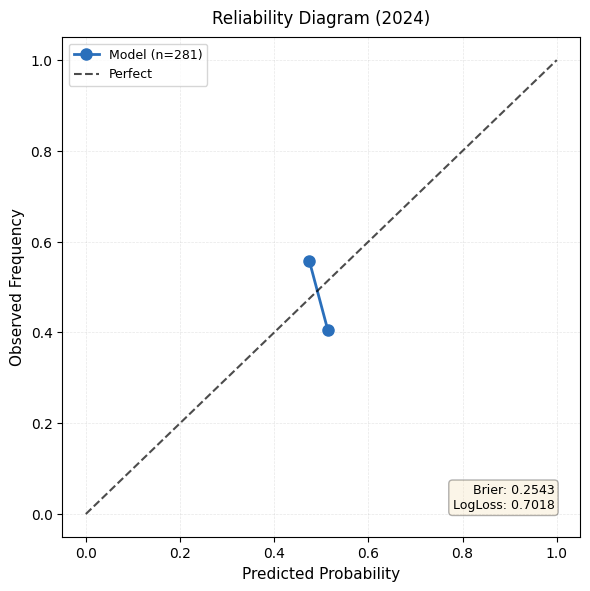
\includegraphics[width=0.48\linewidth]{../figures/out/glm_calibration_platt.png}
    \caption[GLM reliability (Platt)]{Overall reliability curve for GLM with Platt calibration. Circle area proportional to bin count.}
    \label{fig:glm-calibration}
  \end{figure}
}{\begin{center}\textit{[GLM reliability curve will be generated by py/backtest/baseline\_glm.py with --cal-plot]}\end{center}}


\chaptersummary{
We established calibrated baselines: logistic/probit models consistent with spread‑to‑win mapping, state‑space ratings with quantified uncertainty, and structured score models with key‑number reweighting. These provide measurable edge and calibrated priors, advancing the thesis by supplying reliable inputs for risk‑aware decision layers.
}{
\Cref{chap:rl} uses these calibrated signals as inputs to an offline RL framework that turns edge into sequential decisions under safety and governance constraints.
}
